% Plain-language review document (explaneat plain-language review), v5.
\documentclass[a4paper,10pt]{article}
\usepackage[margin=1.8cm]{geometry}
\usepackage{amsmath}
\usepackage{amssymb}
\usepackage{booktabs}
\usepackage{tabularx}
\usepackage{graphicx}
\usepackage[table,usenames,dvipsnames]{xcolor}
\usepackage{tikz}
\usetikzlibrary{arrows.meta,fit,backgrounds,positioning,calc}
\usetikzlibrary{shapes.geometric}
\usepackage{longtable}
\usepackage{pdflscape}
\usepackage{float}
\usepackage[font=small,labelfont=bf]{caption}
\usepackage{array}
\usepackage[unicode=true,hidelinks]{hyperref}
\setcounter{tocdepth}{3}
\setcounter{secnumdepth}{3}
% Review markers, copied from dissertation.tex (7 Nov 2026) for standalone builds.
\newif\ifreviewmarks
\reviewmarkstrue
\newcommand{\reviewrule}{\noindent{\color{BrickRed}\rule{\linewidth}{0.8pt}}}
\newenvironment{drafted}[1][]{%
  \ifreviewmarks\par\addvspace{\medskipamount}\reviewrule\par\nopagebreak
  \noindent{\color{BrickRed}\sffamily\footnotesize\textbf{Thesis Draft}\quad #1\hfill review}\par\nopagebreak\smallskip\fi}{%
  \ifreviewmarks\par\smallskip\noindent{\color{BrickRed}\sffamily\footnotesize end of thesis draft}\par\nopagebreak\reviewrule\par\medskip\fi}
\newcommand{\figreview}[1]{\ifreviewmarks\par\smallskip{\color{NavyBlue}\sffamily\footnotesize\textbf{Figure note:} #1}\par\fi}
\begin{document}
\begin{center}{\Large\bfseries Plain-language explanation: heart-s5-c2\par}\vspace{2mm}{\small AI-assisted drafts for review. Nothing here has been verified by a person.\par}\end{center}
\noindent\textbf{How to read this.} Explanations are built up but read down: the summary first, then each part from the whole model down, in plain words, each sentence followed by the claims it rests on (C01, C02, \ldots; every cited claim was computed on the model and checked). Numbers are changes in predicted risk for a typical patient. The technical record (original hypotheses, formulas, evidence tables with the test check, ranges and n) is at the end. The text describes what the model does, not the world; whether it is plausible is for the reviewer to judge.
\par\medskip\noindent\textbf{What changed in v5e (figures).} v5e: every diagram is a numbered figure with a caption (list of figures after the contents) and the text refers to it; the whole-network figure has its own landscape page, scaled to the page, with a short caption and its description in the text; an input used by several parts is drawn under each of them (same input, repeated for readability, dotted outline); and an appendix figure shows the trained network before any explanation (no parts, no splits).
\par\medskip\noindent\textbf{What changed in v5c (tables and diagrams).} v5c: the evidence tables are landscape, compact and shaded by row, with the header repeated on every page (longtable and pdflscape, used in this review PDF only; the thesis preamble has neither). In the diagrams each input is drawn once, in a shared row along the bottom (the explanation's split copies of an input are listed in the technical detail instead), every cluster has one output rectangle with its plain name, the inputs that feed the output directly meet in a drawn 'sum', and a one-line legend explains the edges.
\par\medskip\noindent\textbf{What changed in v5b (diagrams).} v5b uses one grouping everywhere, the annotation hierarchy: the summary's diagram is the same picture as the whole model's section, and a part that is itself a weighted sum (blood pressure with cholesterol) is a part of its own, described as one that adds up, so the text counts three parts throughout; the lint checks every 'N parts' against the hierarchy. A full-structure diagram follows the summary: every node and connection, nested by part, with the inputs that feed the output directly in their own cluster and the unused input columns listed. Each section from the top down adds its own region of that diagram, with stubs for connections from or to other parts; each connection is drawn in exactly one section. The gate's text now says that it lowers the risk for the patients it acts on, and that more vessels and higher cholesterol take that lowering away; its vessel statements are one per group.
\par\medskip\noindent\textbf{What changed in v5 (read down).} v5 reads the explanation down. The summary (one line, a diagram, one paragraph per block) is as in v4, except that the paragraph on what adds up is split into protective items, risk-raising items and rare results, and an input that also feeds a part is quoted with its direct contribution only (the rest is in that part's paragraph). Then the document walks the annotation hierarchy from the whole model down: for each part a plain hypothesis (what it does for the prediction), plain evidence (what was checked and what it showed; for a part made of others, what they are and how they combine), a diagram one level down and where to read on. The original hypotheses, closed forms and evidence tables are in 'Technical detail' at the end. Statements about structure (what a part is made of, a copy of another part, a formula that reproduces it) are now claims of their own, checked on the graph and the data.
\par\medskip\noindent\textbf{v4.} v4 follows the structure of the explanation. The summary opens with one line and a diagram at the same grouping, then gives one paragraph per top-level block of the annotation hierarchy: one for everything that adds up independently (the inputs that feed the model score directly, and parts that are a weighted sum), and one for each part that combines its inputs in another way: what it combines, how, and for whom. 'Parts in detail' follows the hierarchy below that, with a diagram one level down for each part that contains others. The prose no longer says 'clearly', 'slightly', 'consistently' or 'on the training data only': the numbers carry it, and the test check, the ranges and n stay in the evidence tables. Only genuinely small groups are marked, with their n. The lint rejects the confidence words and checks the block structure.
\tableofcontents
\listoffigures
\clearpage
\begin{drafted}[plain-language layer: heart-s5-c2]
\section{heart-s5-c2}
\noindent{\small Genome \texttt{57c311c6-56f5-4c5d-a475-46433ef58bf2}, explanation \texttt{dabdb4bb-e227-46eb-a995-d4123373f234}. Split: train primary (n=242), test as a check (n=61). Claims: 67, verified 59, not supported 8.\par}
\noindent{\small\textcolor{BrickRed}{AI-assisted draft for review (unverified)}\par}\smallskip
\noindent{\footnotesize Reference (typical) patient: the typical patient: the median training patient for every number and the most common training category for every category (not a real patient). age: 56 years; ca: 0 vessels; chol: 240 mg/dL (6.2 mmol/L); cp: no chest pain (asymptomatic); exang: no chest pain on exercise; fbs: fasting blood sugar of 120 mg/dL or less; oldpeak: 0.8 mm; restecg: a normal resting ECG; sex: male; slope: an upsloping ST segment; thal: a normal thallium scan; thalach: 152 beats per minute; trestbps: 130 mm Hg. Predicted risk of heart disease: 20\%.\par}
\subsection{Summary}
\noindent For a typical patient (a 56-year-old man with no chest pain symptoms and median test results) the model predicts a risk of heart disease of about 20\%; it adds up most of its inputs independently, and five parts add to that sum: a signal from ST depression on exercise and the resting ECG that acts on 109 of 242 training patients, a blood pressure step and a damping term that both read that signal, an extra term for left ventricular hypertrophy without chest pain on exercise, and a very small term for high fasting blood sugar.\,{\scriptsize\textcolor{NavyBlue}{[C34, C42, C53, C61]}} Figure~\ref{fig:hearts5c2:summary} shows the model at this level: one box per paragraph below.
\par\medskip\noindent\fbox{\begin{minipage}{0.96\linewidth}\small\textbf{How to read the diagrams.} Edge colour is the sign of that one connection: blue positive, red negative; thicker is a larger weight. The outline and arrow on an input (and on a part's output box) is its overall effect on the final prediction, read from the verified claims: orange and up arrow raises it, teal and down arrow lowers it, grey and double arrow depends (it goes both ways, or differs between levels). A negative connection into a part that itself raises the prediction means that input lowers the prediction; through a hinge the overall effect can only be read from the claims, not from the edges. Up arrow means towards heart disease; down arrow, away from it. A double outline marks an input (or a part's output) that acts at a fixed rate everywhere: it adds the same amount to the score per unit, so it is explained by its rate alone (see 'Linear factors'); a dashed double outline, at a fixed rate on the observed data. The normal outline is an input whose effect switches on and off somewhere. For example, exercise pain has a negative connection into 'Hypertrophy without exercise pain', a part that raises the predicted risk of heart disease, so exercise pain lowers it.\end{minipage}}\par\medskip
\begin{figure}[H]\centering
\resizebox{!}{\ifdim\height>0.5\textheight 0.5\textheight\else\height\fi}{%
\resizebox{\ifdim\width>\linewidth\linewidth\else\width\fi}{!}{%
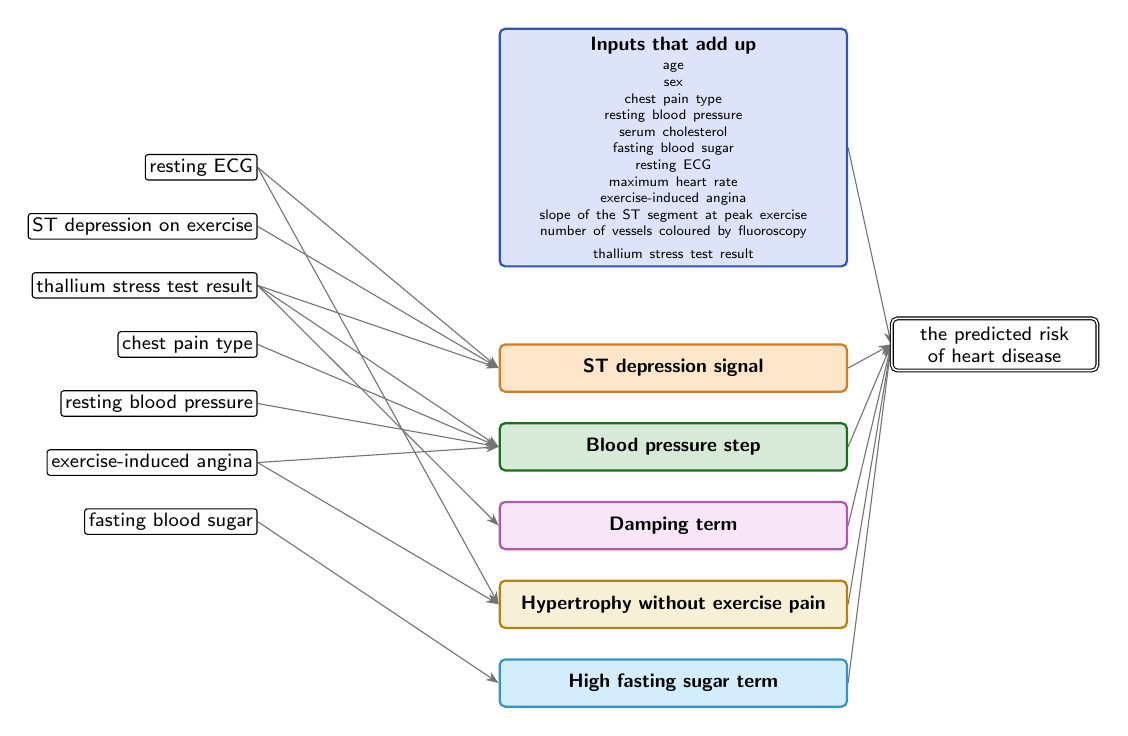
\begin{tikzpicture}[
  font=\sffamily\scriptsize, >={Stealth[length=1.6mm]},
  inp/.style={draw, rounded corners=1pt, fill=white, inner sep=1.5pt, minimum height=3.2mm, anchor=east},
  abox/.style={draw, thick, rounded corners=2pt, align=center, inner sep=3pt, minimum height=6mm, text width=42mm},
  outp/.style={draw, double, rounded corners=2pt, fill=white, align=center, inner sep=3pt, text width=24mm},
  agg/.style={draw=black!55},
]
\node[inp] (i0) at (0,2.25) {resting ECG};
\node[inp] (i1) at (0,1.5) {ST depression on exercise};
\node[inp] (i2) at (0,0.75) {thallium stress test result};
\node[inp] (i3) at (0,-0.0) {chest pain type};
\node[inp] (i4) at (0,-0.75) {resting blood pressure};
\node[inp] (i5) at (0,-1.5) {exercise-induced angina};
\node[inp] (i6) at (0,-2.25) {fasting blood sugar};
\node[abox, fill=RoyalBlue!18, draw=RoyalBlue!80!black] (b0) at (5.28,2.5) {\textbf{Inputs that add up}\\[1pt]{\tiny age\\ sex\\ chest pain type\\ resting blood pressure\\ serum cholesterol\\ fasting blood sugar\\ resting ECG\\ maximum heart rate\\ exercise-induced angina\\ slope of the ST segment at peak exercise\\ number of vessels coloured by fluoroscopy\\ thallium stress test result}};
\node[abox, fill=BurntOrange!18, draw=BurntOrange!80!black] (b1) at (5.28,-0.3) {\textbf{ST depression signal}};
\node[abox, fill=ForestGreen!18, draw=ForestGreen!80!black] (b2) at (5.28,-1.3) {\textbf{Blood pressure step}};
\node[abox, fill=Orchid!18, draw=Orchid!80!black] (b3) at (5.28,-2.3) {\textbf{Damping term}};
\node[abox, fill=Goldenrod!18, draw=Goldenrod!80!black] (b4) at (5.28,-3.3) {\textbf{Hypertrophy without exercise pain}};
\node[abox, fill=Cerulean!18, draw=Cerulean!80!black] (b5) at (5.28,-4.3) {\textbf{High fasting sugar term}};
\node[outp] (out) at (9.36,0) {the predicted risk of heart disease};
\begin{scope}[on background layer]
\draw[->, agg] (b0.east) -- (out.west);
\draw[->, agg, thin] (i0.east) -- (b1.west);
\draw[->, agg, thin] (i1.east) -- (b1.west);
\draw[->, agg, thin] (i2.east) -- (b1.west);
\draw[->, agg] (b1.east) -- (out.west);
\draw[->, agg, thin] (i3.east) -- (b2.west);
\draw[->, agg, thin] (i4.east) -- (b2.west);
\draw[->, agg, thin] (i5.east) -- (b2.west);
\draw[->, agg, thin] (i2.east) -- (b2.west);
\draw[->, agg] (b2.east) -- (out.west);
\draw[->, agg, thin] (i2.east) -- (b3.west);
\draw[->, agg] (b3.east) -- (out.west);
\draw[->, agg, thin] (i0.east) -- (b4.west);
\draw[->, agg, thin] (i5.east) -- (b4.west);
\draw[->, agg] (b4.east) -- (out.west);
\draw[->, agg, thin] (i6.east) -- (b5.west);
\draw[->, agg] (b5.east) -- (out.west);
\end{scope}
\end{tikzpicture}}}%
\caption{The model at the level of the summary: one box per part.}
\label{fig:hearts5c2:summary}
\end{figure}
\paragraph{Inputs that add up.} \par\noindent\textit{Lowering the risk.}  These add up independently, and these lower the risk: being a woman takes a typical patient's predicted risk from about 20\% to about 3\%; through this sum alone typical angina lowers it to about 2\%, non-anginal chest pain to about 4\%, fasting blood sugar above 120 mg/dL to about 10\% and atypical angina to about 11\%; and a higher maximum heart rate lowers it steadily, from about 26\% at 118 to about 16\% at 175 beats per minute.\,{\scriptsize\textcolor{NavyBlue}{[C08, C06, C12, C18, C20, C19]}} \par\noindent\textit{Raising the risk.}  Each extra vessel coloured by fluoroscopy adds about the same, from about 20\% at 0 to about 87\% at 2 vessels, flattening out near the top because the predicted risk cannot go much higher; a flat rather than upsloping ST segment raises it to about 61\%, higher cholesterol raises it steadily from about 13\% at 193 mg/dL to about 34\% at 308 mg/dL, and older age raises it steadily from about 17\% at 42 to about 22\% at 66 years.\,{\scriptsize\textcolor{NavyBlue}{[C01, C02, C04, C27]}} Through this sum alone, higher resting blood pressure raises it steadily, from about 12\% at 110 mm Hg to about 33\% at 155 mm Hg, a thallium result other than a normal scan or a fixed defect raises it to about 36\%, chest pain brought on by exercise raises it to about 33\%, and a resting ECG other than normal raises it to about 25\%; all four also act through the parts below.\,{\scriptsize\textcolor{NavyBlue}{[C05, C09, C14, C26]}} \par\noindent\textit{Rare results.}  Some rarer results also count (the model has little data on this, n = 15 to 17): through this sum alone a fixed defect on the thallium scan lowers the risk to about 9\%, and a downsloping ST segment raises it to about 27\%.\,{\scriptsize\textcolor{NavyBlue}{[C17, C24]}}
\paragraph{ST depression signal.} This part reads ST depression on exercise, the resting ECG and the thallium scan, and acts on 109 of 242 training patients, 65 of whom had heart disease; for the typical patient it acts on, the predicted risk is about 76\% without it and about 89\% with it.\,{\scriptsize\textcolor{NavyBlue}{[C42]}} Through it, more ST depression adds to the predicted risk only once it rises above about 1.3 mm (between 0.4 and 1.3 mm for different patients), rising in an uneven way: for a typical patient from about 16\% at 0 mm to about 50\% at 2.8 mm.\,{\scriptsize\textcolor{NavyBlue}{[C35, C41]}} ST depression counts more with a normal resting ECG (from about 16\% to about 50\%) than with any other resting ECG (from about 25\% to about 48\%), in an uneven way.\,{\scriptsize\textcolor{NavyBlue}{[C39]}} Through it, a resting ECG other than normal lowers a typical patient's risk from about 20\% to about 16\%, and a thallium result coded 4 shuts the signal (the model has little data on this, n = 2).\,{\scriptsize\textcolor{NavyBlue}{[C36, C37]}}
\paragraph{Blood pressure step.} This part reads that signal together with resting blood pressure, chest pain on exercise and chest pain type, and acts on 145 of 242 training patients, 73 of whom had heart disease; for the typical patient it acts on, the predicted risk is about 51\% without it and about 68\% with it.\,{\scriptsize\textcolor{NavyBlue}{[C53]}} Through it, higher resting blood pressure lowers the risk up to about 125 mm Hg (between 122 and 165 mm Hg for different patients), then no further, in an uneven way: for a typical patient from about 23\% at 110 mm Hg to about 17\% at 155 mm Hg.\,{\scriptsize\textcolor{NavyBlue}{[C44, C52]}} Through it, chest pain on exercise lowers a typical patient's risk from about 20\% to about 18\%, and non-anginal chest pain to about 19\%.\,{\scriptsize\textcolor{NavyBlue}{[C45, C46]}}
\paragraph{Damping term.} This part reads the same signal and the thallium scan, and acts on 234 of 242 training patients, 102 of whom had heart disease; for the typical patient it acts on, the predicted risk is about 24\% without it and about 20\% with it.\,{\scriptsize\textcolor{NavyBlue}{[C56]}} Through it, a fixed defect on the thallium scan raises a typical patient's risk from about 20\% to about 23\% (the model has little data on this, n = 15).\,{\scriptsize\textcolor{NavyBlue}{[C55]}}
\paragraph{Hypertrophy without exercise pain.} This part acts on 74 of 242 training patients, nearly all with left ventricular hypertrophy on the resting ECG and no chest pain on exercise, 30 of whom had heart disease; for the typical patient it acts on, the predicted risk is about 25\% without it and about 30\% with it.\,{\scriptsize\textcolor{NavyBlue}{[C61]}} Through it, left ventricular hypertrophy raises a typical patient's risk from about 20\% to about 24\%, and for the typical patient it acts on, chest pain on exercise lowers it from about 30\% to about 25\%.\,{\scriptsize\textcolor{NavyBlue}{[C59, C58]}} Across the model, chest pain on exercise raises a typical patient's risk from about 20\% to about 31\% without left ventricular hypertrophy, and from about 25\% to about 35\% with it.\,{\scriptsize\textcolor{NavyBlue}{[C60]}}
\paragraph{High fasting sugar term.} This part acts on 33 of 242 training patients, nearly all with fasting blood sugar above 120 mg/dL, 15 of whom had heart disease; for the typical patient it acts on, the predicted risk is about 24\% without it and about 25\% with it.\,{\scriptsize\textcolor{NavyBlue}{[C65]}} It barely changes the predictions, by at most 2 percentage points.\,{\scriptsize\textcolor{NavyBlue}{[C66]}}
\paragraph{The whole network.} Figure~\ref{fig:hearts5c2:overview} (next page, landscape) draws every unit and connection of the explained model, nested by part: shaded clusters are the parts of the model and darker boxes the parts inside them; circles are hidden units (h1, h2, \ldots); each cluster's rectangle is its output, and a dashed `sum' stands for an addition the next unit does (drawn, not a unit of the model); the hexagon is the model's output. An input used by several parts is drawn under each of them (same label, dotted outline, the first copy marked with the number of copies): it is the same input, repeated for readability. Not used by the model (input columns with no connection): male, atypical angina, ST-T abnormal ECG, flat ST, reversible defect.
\begin{landscape}
\begin{figure}[p]\centering
\resizebox{\linewidth}{!}{%
\definecolor{netup}{HTML}{D95F02}\definecolor{netdown}{HTML}{1B9E77}\definecolor{netmixed}{HTML}{7F7F7F}%
\begin{tikzpicture}[
  font=\sffamily\scriptsize, >={Stealth[length=1.4mm]},
  inp/.style={draw, circle, fill=white, minimum size=3.2mm, inner sep=0pt},
  hid/.style={draw, circle, fill=white, minimum size=5.2mm, inner sep=0.5pt, font=\sffamily\tiny},
  exitbox/.style={draw, thick, rectangle, fill=white, align=center, text width=17mm, minimum height=5mm, inner sep=1.5pt, font=\sffamily\tiny},
  sumbox/.style={draw, thick, dashed, rectangle, fill=white, align=center, text width=17mm, minimum height=5mm, inner sep=1.5pt, font=\sffamily\tiny},
  outp/.style={draw, thick, regular polygon, regular polygon sides=6, fill=white, minimum size=10mm, inner sep=0pt, font=\sffamily\tiny, align=center},
  stub/.style={draw, dashed, rounded corners=2pt, fill=white, align=center, inner sep=2pt, font=\sffamily\tiny, text width=15mm},
  inlab/.style={font=\sffamily\tiny, align=center, text width=15mm, inner sep=1pt, fill=white, fill opacity=0.8, text opacity=1},
  wpos/.style={draw=NavyBlue}, wneg/.style={draw=BrickRed}, wagg/.style={draw=black!45, line width=1.2pt},
  wmix/.style={draw=Plum},
]
\node[outp] (n0) at (22.1,6.15) {heart disease};
\node[exitbox] (n1416) at (30.12,4.6) {Damping term $\downarrow$};
\node[exitbox] (n1611) at (36.16,1.9) {Hypertrophy without exercise pain $\uparrow$};
\node[exitbox] (n204) at (15.94,1.9) {ST depression signal $\updownarrow$};
\node[exitbox] (n290) at (23.78,4.6) {Blood pressure step $\uparrow$};
\node[exitbox] (n3884) at (43.3,1.9) {High fasting sugar term $\uparrow$};
\node[hid] (nidentityx1416) at (30.12,3.25) {h7};
\node[hid] (nidentityx290) at (23.78,3.25) {h6};
\node[sumbox] (nxxsumxx) at (5.85,1.9) {sum: Inputs that add up};
\node[inp, draw=netup, very thick] (ninxxagexxadditive) at (0.9,0.0) {};
\path (ninxxagexxadditive.south) node[inlab, anchor=north] (labninxxagexxadditive) {age $\uparrow$};
\node[inp, draw=netdown, very thick] (ninxxsexx0xxadditive) at (3.6,-1.05) {};
\path (ninxxsexx0xxadditive.south) node[inlab, anchor=north] (labninxxsexx0xxadditive) {female $\downarrow$};
\node[inp, draw=netdown, very thick] (ninxxcpx1xxadditive) at (9.0,-1.05) {};
\path (ninxxcpx1xxadditive.south) node[inlab, anchor=north] (labninxxcpx1xxadditive) {typical angina $\downarrow$};
\node[inp, draw=netup, very thick] (ninxxcpx4xxadditive) at (5.4,-1.05) {};
\path (ninxxcpx4xxadditive.south) node[inlab, anchor=north] (labninxxcpx4xxadditive) {no chest pain $\uparrow$};
\node[inp, draw=netup, very thick] (ninxxcholxxadditive) at (1.8,-1.05) {};
\path (ninxxcholxxadditive.south) node[inlab, anchor=north] (labninxxcholxxadditive) {cholesterol $\uparrow$};
\node[inp, draw=netup, very thick] (ninxxfbsx0xxadditive) at (8.1,-2.1) {};
\path (ninxxfbsx0xxadditive.south) node[inlab, anchor=north] (labninxxfbsx0xxadditive) {sugar 120 or less $\uparrow$};
\node[inp, draw=netdown, very thick] (ninxxthalachxxadditive) at (4.5,-2.1) {};
\path (ninxxthalachxxadditive.south) node[inlab, anchor=north] (labninxxthalachxxadditive) {max heart rate $\downarrow$};
\node[inp, draw=netdown, very thick] (ninxxexangx0xxadditive) at (6.3,0.0) {};
\path (ninxxexangx0xxadditive.south) node[inlab, anchor=north] (labninxxexangx0xxadditive) {no exercise pain $\downarrow$};
\node[inp, draw=netdown, very thick] (ninxxslopex1xxadditive) at (9.9,0.0) {};
\path (ninxxslopex1xxadditive.south) node[inlab, anchor=north] (labninxxslopex1xxadditive) {upsloping ST $\downarrow$};
\node[inp, draw=netup, very thick] (ninxxslopex3xxadditive) at (2.7,0.0) {};
\path (ninxxslopex3xxadditive.south) node[inlab, anchor=north] (labninxxslopex3xxadditive) {downsloping ST $\uparrow$};
\node[inp, draw=netup, very thick] (ninxxcaxxadditive) at (10.8,-1.05) {};
\path (ninxxcaxxadditive.south) node[inlab, anchor=north] (labninxxcaxxadditive) {vessels $\uparrow$};
\node[inp, draw=netmixed, very thick] (ninxxthalx3xxadditive) at (8.1,0.0) {};
\path (ninxxthalx3xxadditive.south) node[inlab, anchor=north] (labninxxthalx3xxadditive) {normal thallium $\updownarrow$};
\node[inp, draw=netup, very thick] (ninxxoldpeakxxannx33) at (14.14,0.0) {};
\path (ninxxoldpeakxxannx33.south) node[inlab, anchor=north] (labninxxoldpeakxxannx33) {ST depression $\uparrow$};
\node[inp, draw=netdown, very thick] (ninxxthalx4xxannx33) at (17.74,0.0) {};
\path (ninxxthalx4xxannx33.south) node[inlab, anchor=north] (labninxxthalx4xxannx33) {thallium code 4 $\downarrow$};
\node[inp, draw=netup, very thick] (ninxxfbsx1xxannx37) at (43.3,0.0) {};
\path (ninxxfbsx1xxannx37.south) node[inlab, anchor=north] (labninxxfbsx1xxannx37) {sugar above 120 $\uparrow$};
\node[inp, draw=netup, very thick] (ninxxrestecgx2xxannx36) at (35.26,0.0) {};
\path (ninxxrestecgx2xxannx36.south) node[inlab, anchor=north] (labninxxrestecgx2xxannx36) {LVH on ECG $\uparrow$};
\node[inp, densely dotted, thick, draw=netdown, very thick] (ninxxrestecgx0xxadditive) at (7.2,-1.05) {};
\path (ninxxrestecgx0xxadditive.south) node[inlab, anchor=north] (labninxxrestecgx0xxadditive) {normal ECG ($\times$2) $\downarrow$};
\node[inp, densely dotted, thick, draw=netup, very thick] (ninxxrestecgx0xxannx33) at (15.94,0.0) {};
\path (ninxxrestecgx0xxannx33.south) node[inlab, anchor=north] (labninxxrestecgx0xxannx33) {normal ECG $\uparrow$};
\node[inp, densely dotted, thick, draw=netup, very thick] (ninxxexangx1xxadditive) at (2.7,-2.1) {};
\path (ninxxexangx1xxadditive.south) node[inlab, anchor=north] (labninxxexangx1xxadditive) {exercise pain ($\times$3) $\uparrow$};
\node[inp, densely dotted, thick, draw=netdown, very thick] (ninxxexangx1xxannx34) at (22.88,0.0) {};
\path (ninxxexangx1xxannx34.south) node[inlab, anchor=north] (labninxxexangx1xxannx34) {exercise pain $\downarrow$};
\node[inp, densely dotted, thick, draw=netdown, very thick] (ninxxexangx1xxannx36) at (37.06,0.0) {};
\path (ninxxexangx1xxannx36.south) node[inlab, anchor=north] (labninxxexangx1xxannx36) {exercise pain $\downarrow$};
\node[inp, densely dotted, thick, draw=netdown, very thick] (ninxxthalx6xxadditive) at (4.5,0.0) {};
\path (ninxxthalx6xxadditive.south) node[inlab, anchor=north] (labninxxthalx6xxadditive) {fixed defect ($\times$3) $\downarrow$};
\node[inp, densely dotted, thick, draw=netdown, very thick] (ninxxthalx6xxannx34) at (24.68,0.0) {};
\path (ninxxthalx6xxannx34.south) node[inlab, anchor=north] (labninxxthalx6xxannx34) {fixed defect $\downarrow$};
\node[inp, densely dotted, thick, draw=netup, very thick] (ninxxthalx6xxannx35) at (30.12,0.0) {};
\path (ninxxthalx6xxannx35.south) node[inlab, anchor=north] (labninxxthalx6xxannx35) {fixed defect $\uparrow$};
\node[inp, densely dotted, thick, draw=netup, very thick] (ninxxtrestbpsxxadditive) at (0.9,-2.1) {};
\path (ninxxtrestbpsxxadditive.south) node[inlab, anchor=north] (labninxxtrestbpsxxadditive) {blood pressure ($\times$2) $\uparrow$};
\node[inp, densely dotted, thick, draw=netdown, very thick] (ninxxtrestbpsxxannx34) at (21.08,0.0) {};
\path (ninxxtrestbpsxxannx34.south) node[inlab, anchor=north] (labninxxtrestbpsxxannx34) {blood pressure $\downarrow$};
\node[inp, densely dotted, thick, draw=netdown, very thick] (ninxxcpx3xxadditive) at (6.3,-2.1) {};
\path (ninxxcpx3xxadditive.south) node[inlab, anchor=north] (labninxxcpx3xxadditive) {non-anginal pain ($\times$2) $\downarrow$};
\node[inp, densely dotted, thick, draw=netdown, very thick] (ninxxcpx3xxannx34) at (26.48,0.0) {};
\path (ninxxcpx3xxannx34.south) node[inlab, anchor=north] (labninxxcpx3xxannx34) {non-anginal pain $\downarrow$};
\begin{scope}[on background layer]
\node[fit=(nxxsumxx) , inner sep=8pt, rounded corners=5pt, fill=RoyalBlue!10, draw=RoyalBlue!45] (clu0) {};
\node[fit=(n204) , inner sep=8pt, rounded corners=5pt, fill=BurntOrange!10, draw=BurntOrange!45] (clu1) {};
\node[fit=(n290) (nidentityx290) , inner sep=8pt, rounded corners=5pt, fill=ForestGreen!10, draw=ForestGreen!45] (clu2) {};
\node[fit=(n1416) (nidentityx1416) , inner sep=8pt, rounded corners=5pt, fill=Orchid!10, draw=Orchid!45] (clu3) {};
\node[fit=(n1611) , inner sep=8pt, rounded corners=5pt, fill=Goldenrod!10, draw=Goldenrod!45] (clu4) {};
\node[fit=(n3884) , inner sep=8pt, rounded corners=5pt, fill=Cerulean!10, draw=Cerulean!45] (clu5) {};
\draw[->, wpos, line width=0.29pt] (ninxxagexxadditive) -- (nxxsumxx);
\draw[->, wneg, line width=0.62pt] (ninxxsexx0xxadditive) -- (nxxsumxx);
\draw[->, wneg, line width=0.42pt] (ninxxcpx1xxadditive) -- (nxxsumxx);
\draw[->, wpos, line width=0.38pt] (ninxxcpx4xxadditive) -- (nxxsumxx);
\draw[->, wpos, line width=0.43pt] (ninxxcholxxadditive) -- (nxxsumxx);
\draw[->, wpos, line width=0.34pt] (ninxxfbsx0xxadditive) -- (nxxsumxx);
\draw[->, wneg, line width=0.33pt] (ninxxthalachxxadditive) -- (nxxsumxx);
\draw[->, wpos, line width=0.30pt] (ninxxexangx0xxadditive) -- (nxxsumxx);
\draw[->, wneg, line width=0.57pt] (ninxxslopex1xxadditive) -- (nxxsumxx);
\draw[->, wneg, line width=0.38pt] (ninxxslopex3xxadditive) -- (nxxsumxx);
\draw[->, wpos, line width=0.77pt] (ninxxcaxxadditive) -- (nxxsumxx);
\draw[->, wneg, line width=0.40pt] (ninxxthalx3xxadditive) -- (nxxsumxx);
\draw[->, wpos, line width=0.30pt] (n204) -- (n0);
\draw[->, wpos, line width=0.34pt] (n290) -- (n0);
\draw[->, wneg, line width=0.29pt] (n1416) -- (n0);
\draw[->, wpos, line width=0.51pt] (n1611) -- (n0);
\draw[->, wpos, line width=0.27pt] (n3884) -- (n0);
\draw[->, wpos, line width=1.14pt] (ninxxoldpeakxxannx33) -- (n204);
\draw[->, wneg, line width=0.56pt] (ninxxthalx4xxannx33) -- (n204);
\draw[->, wpos, line width=0.60pt] (ninxxfbsx1xxannx37) -- (n3884);
\draw[->, wpos, line width=0.56pt] (ninxxrestecgx2xxannx36) -- (n1611);
\draw[->, wneg, line width=0.31pt] (ninxxrestecgx0xxadditive) -- (nxxsumxx);
\draw[->, wpos, line width=0.60pt] (ninxxrestecgx0xxannx33) -- (n204);
\draw[->, wpos, line width=0.41pt] (ninxxexangx1xxadditive) -- (nxxsumxx);
\draw[->, wneg, line width=0.30pt] (ninxxexangx1xxannx34) -- (n290);
\draw[->, wneg, line width=0.58pt] (ninxxexangx1xxannx36) -- (n1611);
\draw[->, wneg, line width=0.39pt] (ninxxthalx6xxadditive) -- (nxxsumxx);
\draw[->, wneg, line width=0.25pt] (ninxxthalx6xxannx34) -- (n290);
\draw[->, wneg, line width=0.46pt] (ninxxthalx6xxannx35) -- (n1416);
\draw[->, wpos, line width=0.42pt] (ninxxtrestbpsxxadditive) -- (nxxsumxx);
\draw[->, wneg, line width=0.52pt] (ninxxtrestbpsxxannx34) -- (n290);
\draw[->, wneg, line width=0.41pt] (ninxxcpx3xxadditive) -- (nxxsumxx);
\draw[->, wneg, line width=0.27pt] (ninxxcpx3xxannx34) -- (n290);
\draw[->, wpos, line width=0.65pt] (n204) -- (nidentityx290);
\draw[->, wpos, line width=0.60pt] (nidentityx290) -- (n290);
\draw[->, wpos, line width=0.54pt] (n204) -- (nidentityx1416);
\draw[->, wpos, line width=0.60pt] (nidentityx1416) -- (n1416);
\draw[->, wagg] (nxxsumxx) -- (n0);
\end{scope}
\node[font=\sffamily\scriptsize\bfseries, text=RoyalBlue!55!black, anchor=south west, inner sep=1pt, fill=white, fill opacity=0.85, text opacity=1] at (clu0.north west) {Inputs that add up};
\node[font=\sffamily\scriptsize\bfseries, text=BurntOrange!55!black, anchor=south west, inner sep=1pt, fill=white, fill opacity=0.85, text opacity=1] at (clu1.north west) {ST depression signal};
\node[font=\sffamily\scriptsize\bfseries, text=ForestGreen!55!black, anchor=south west, inner sep=1pt, fill=white, fill opacity=0.85, text opacity=1] at (clu2.north west) {Blood pressure step};
\node[font=\sffamily\scriptsize\bfseries, text=Orchid!55!black, anchor=south west, inner sep=1pt, fill=white, fill opacity=0.85, text opacity=1] at (clu3.north west) {Damping term};
\node[font=\sffamily\scriptsize\bfseries, text=Goldenrod!55!black, anchor=south west, inner sep=1pt, fill=white, fill opacity=0.85, text opacity=1] at (clu4.north west) {Hypertrophy without exercise pain};
\node[font=\sffamily\scriptsize\bfseries, text=Cerulean!55!black, anchor=south west, inner sep=1pt, fill=white, fill opacity=0.85, text opacity=1] at (clu5.north west) {High fasting sugar term};
\end{tikzpicture}}%
\caption{Every unit and connection of the explained model, nested by part. Blue: positive weight (raises the score); red: negative weight (lowers it); thicker: larger weight. Orange outline and up arrow: raises the final prediction; teal and down arrow: lowers it; grey and double arrow: depends.}
\label{fig:hearts5c2:overview}
\end{figure}
\end{landscape}
\paragraph{Worth checking against what is known.} Worth checking: the model treats fasting blood sugar above 120 mg/dL as lowering the risk of heart disease (for a typical patient from about 20\% to about 11\%).\,{\scriptsize\textcolor{NavyBlue}{[C22]}} Worth checking: patients with typical angina get the lowest predicted risk of all chest pain types, below patients with no chest pain symptoms.\,{\scriptsize\textcolor{NavyBlue}{[C07, C11, C21]}} Worth checking: the model treats a fixed defect on the thallium scan as lowering the risk compared with a normal scan, from only 15 training patients.\,{\scriptsize\textcolor{NavyBlue}{[C23]}} Worth checking: ST depression on exercise raises the predicted risk more when the resting ECG is normal than when it is not.\,{\scriptsize\textcolor{NavyBlue}{[C39]}} Worth checking: through the blood pressure step, higher resting blood pressure lowers the predicted risk, against its rise through the sum.\,{\scriptsize\textcolor{NavyBlue}{[C44, C05]}} Worth checking: for the 2 training patients whose thallium result is coded 4, a code the dataset documentation does not define, the ST depression signal is shut.\,{\scriptsize\textcolor{NavyBlue}{[C37]}}
\subsection{The model, read from the top down}
\noindent{\small Each part of the explanation in turn, from the whole model down to the smallest parts: what it does for the prediction (hypothesis), what was checked (evidence), a diagram one level down, and where to read on. The technical record of each part is in ``Technical detail'' at the end.\par}
\subsubsection{The whole model}\label{rd:ann38}
\noindent{\small Figure~\ref{fig:hearts5c2:parts-ann38} shows what feeds this part; Figure~\ref{fig:hearts5c2:units-ann38} its units and every connection into them (dashed boxes: connections from or to other parts, drawn in their own sections).\par}
\begin{figure}[H]\centering
\resizebox{!}{\ifdim\height>0.5\textheight 0.5\textheight\else\height\fi}{%
\resizebox{\ifdim\width>\linewidth\linewidth\else\width\fi}{!}{%
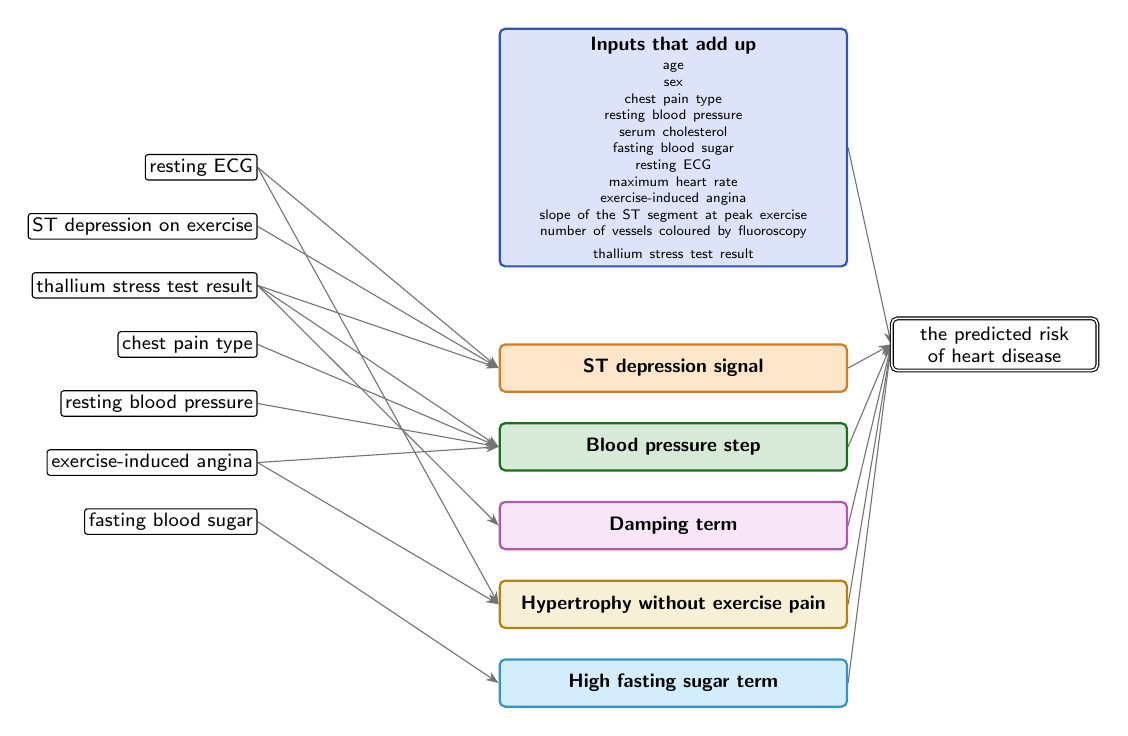
\begin{tikzpicture}[
  font=\sffamily\scriptsize, >={Stealth[length=1.6mm]},
  inp/.style={draw, rounded corners=1pt, fill=white, inner sep=1.5pt, minimum height=3.2mm, anchor=east},
  abox/.style={draw, thick, rounded corners=2pt, align=center, inner sep=3pt, minimum height=6mm, text width=42mm},
  outp/.style={draw, double, rounded corners=2pt, fill=white, align=center, inner sep=3pt, text width=24mm},
  agg/.style={draw=black!55},
]
\node[inp] (i0) at (0,2.25) {resting ECG};
\node[inp] (i1) at (0,1.5) {ST depression on exercise};
\node[inp] (i2) at (0,0.75) {thallium stress test result};
\node[inp] (i3) at (0,-0.0) {chest pain type};
\node[inp] (i4) at (0,-0.75) {resting blood pressure};
\node[inp] (i5) at (0,-1.5) {exercise-induced angina};
\node[inp] (i6) at (0,-2.25) {fasting blood sugar};
\node[abox, fill=RoyalBlue!18, draw=RoyalBlue!80!black] (b0) at (5.28,2.5) {\textbf{Inputs that add up}\\[1pt]{\tiny age\\ sex\\ chest pain type\\ resting blood pressure\\ serum cholesterol\\ fasting blood sugar\\ resting ECG\\ maximum heart rate\\ exercise-induced angina\\ slope of the ST segment at peak exercise\\ number of vessels coloured by fluoroscopy\\ thallium stress test result}};
\node[abox, fill=BurntOrange!18, draw=BurntOrange!80!black] (b1) at (5.28,-0.3) {\textbf{ST depression signal}};
\node[abox, fill=ForestGreen!18, draw=ForestGreen!80!black] (b2) at (5.28,-1.3) {\textbf{Blood pressure step}};
\node[abox, fill=Orchid!18, draw=Orchid!80!black] (b3) at (5.28,-2.3) {\textbf{Damping term}};
\node[abox, fill=Goldenrod!18, draw=Goldenrod!80!black] (b4) at (5.28,-3.3) {\textbf{Hypertrophy without exercise pain}};
\node[abox, fill=Cerulean!18, draw=Cerulean!80!black] (b5) at (5.28,-4.3) {\textbf{High fasting sugar term}};
\node[outp] (out) at (9.36,0) {the predicted risk of heart disease};
\begin{scope}[on background layer]
\draw[->, agg] (b0.east) -- (out.west);
\draw[->, agg, thin] (i0.east) -- (b1.west);
\draw[->, agg, thin] (i1.east) -- (b1.west);
\draw[->, agg, thin] (i2.east) -- (b1.west);
\draw[->, agg] (b1.east) -- (out.west);
\draw[->, agg, thin] (i3.east) -- (b2.west);
\draw[->, agg, thin] (i4.east) -- (b2.west);
\draw[->, agg, thin] (i5.east) -- (b2.west);
\draw[->, agg, thin] (i2.east) -- (b2.west);
\draw[->, agg] (b2.east) -- (out.west);
\draw[->, agg, thin] (i2.east) -- (b3.west);
\draw[->, agg] (b3.east) -- (out.west);
\draw[->, agg, thin] (i0.east) -- (b4.west);
\draw[->, agg, thin] (i5.east) -- (b4.west);
\draw[->, agg] (b4.east) -- (out.west);
\draw[->, agg, thin] (i6.east) -- (b5.west);
\draw[->, agg] (b5.east) -- (out.west);
\end{scope}
\end{tikzpicture}}}%
\caption{The whole model: what feeds it, one level down.}
\label{fig:hearts5c2:parts-ann38}
\end{figure}
\begin{figure}[H]\centering
\resizebox{\ifdim\width>\linewidth\linewidth\else\width\fi}{!}{%
\definecolor{netup}{HTML}{D95F02}\definecolor{netdown}{HTML}{1B9E77}\definecolor{netmixed}{HTML}{7F7F7F}%
\begin{tikzpicture}[
  font=\sffamily\scriptsize, >={Stealth[length=1.4mm]},
  inp/.style={draw, circle, fill=white, minimum size=3.2mm, inner sep=0pt},
  hid/.style={draw, circle, fill=white, minimum size=5.2mm, inner sep=0.5pt, font=\sffamily\tiny},
  exitbox/.style={draw, thick, rectangle, fill=white, align=center, text width=17mm, minimum height=5mm, inner sep=1.5pt, font=\sffamily\tiny},
  sumbox/.style={draw, thick, dashed, rectangle, fill=white, align=center, text width=17mm, minimum height=5mm, inner sep=1.5pt, font=\sffamily\tiny},
  outp/.style={draw, thick, regular polygon, regular polygon sides=6, fill=white, minimum size=10mm, inner sep=0pt, font=\sffamily\tiny, align=center},
  stub/.style={draw, dashed, rounded corners=2pt, fill=white, align=center, inner sep=2pt, font=\sffamily\tiny, text width=15mm},
  inlab/.style={font=\sffamily\tiny, align=center, text width=15mm, inner sep=1pt, fill=white, fill opacity=0.8, text opacity=1},
  wpos/.style={draw=NavyBlue}, wneg/.style={draw=BrickRed}, wagg/.style={draw=black!45, line width=1.2pt},
  wmix/.style={draw=Plum},
]
\node[outp] (n0) at (11.12,3.45) {heart disease};
\node[inp, draw=netup, very thick] (ninxxage) at (0.9,0.0) {};
\path (ninxxage.south) node[inlab, anchor=north] (labninxxage) {age $\uparrow$};
\node[sumbox] (nxxsumxx) at (5.85,1.9) {sum: Inputs that add up};
\node[inp, draw=netdown, very thick] (ninxxsexx0) at (3.6,-1.05) {};
\path (ninxxsexx0.south) node[inlab, anchor=north] (labninxxsexx0) {female $\downarrow$};
\node[inp, draw=netdown, very thick] (ninxxcpx1) at (9.0,-1.05) {};
\path (ninxxcpx1.south) node[inlab, anchor=north] (labninxxcpx1) {typical angina $\downarrow$};
\node[inp, draw=netup, very thick] (ninxxcpx4) at (5.4,-1.05) {};
\path (ninxxcpx4.south) node[inlab, anchor=north] (labninxxcpx4) {no chest pain $\uparrow$};
\node[inp, draw=netup, very thick] (ninxxchol) at (1.8,-1.05) {};
\path (ninxxchol.south) node[inlab, anchor=north] (labninxxchol) {cholesterol $\uparrow$};
\node[inp, draw=netup, very thick] (ninxxfbsx0) at (8.1,-2.1) {};
\path (ninxxfbsx0.south) node[inlab, anchor=north] (labninxxfbsx0) {sugar 120 or less $\uparrow$};
\node[inp, draw=netdown, very thick] (ninxxthalach) at (4.5,-2.1) {};
\path (ninxxthalach.south) node[inlab, anchor=north] (labninxxthalach) {max heart rate $\downarrow$};
\node[inp, draw=netdown, very thick] (ninxxexangx0) at (6.3,0.0) {};
\path (ninxxexangx0.south) node[inlab, anchor=north] (labninxxexangx0) {no exercise pain $\downarrow$};
\node[inp, draw=netdown, very thick] (ninxxslopex1) at (9.9,0.0) {};
\path (ninxxslopex1.south) node[inlab, anchor=north] (labninxxslopex1) {upsloping ST $\downarrow$};
\node[inp, draw=netup, very thick] (ninxxslopex3) at (2.7,0.0) {};
\path (ninxxslopex3.south) node[inlab, anchor=north] (labninxxslopex3) {downsloping ST $\uparrow$};
\node[inp, draw=netup, very thick] (ninxxca) at (10.8,-1.05) {};
\path (ninxxca.south) node[inlab, anchor=north] (labninxxca) {vessels $\uparrow$};
\node[inp, draw=netmixed, very thick] (ninxxthalx3) at (8.1,0.0) {};
\path (ninxxthalx3.south) node[inlab, anchor=north] (labninxxthalx3) {normal thallium $\updownarrow$};
\node[stub] (nfromxxSTxdepressionxsignal) at (21.34,0.0) {from ST depression signal};
\node[stub] (nfromxxBloodxpressurexstep) at (14.14,0.0) {from Blood pressure step};
\node[stub] (nfromxxDampingxterm) at (15.94,0.0) {from Damping term};
\node[stub] (nfromxxHypertrophyxwithoutxexercisexpain) at (19.54,0.0) {from Hypertrophy without exercise pain};
\node[stub] (nfromxxHighxfastingxsugarxterm) at (17.74,0.0) {from High fasting sugar term};
\node[inp, draw=netdown, very thick] (ninxxrestecgx0) at (7.2,-1.05) {};
\path (ninxxrestecgx0.south) node[inlab, anchor=north] (labninxxrestecgx0) {normal ECG $\downarrow$};
\node[inp, draw=netup, very thick] (ninxxexangx1) at (2.7,-2.1) {};
\path (ninxxexangx1.south) node[inlab, anchor=north] (labninxxexangx1) {exercise pain $\uparrow$};
\node[inp, draw=netdown, very thick] (ninxxthalx6) at (4.5,0.0) {};
\path (ninxxthalx6.south) node[inlab, anchor=north] (labninxxthalx6) {fixed defect $\downarrow$};
\node[inp, draw=netup, very thick] (ninxxtrestbps) at (0.9,-2.1) {};
\path (ninxxtrestbps.south) node[inlab, anchor=north] (labninxxtrestbps) {blood pressure $\uparrow$};
\node[inp, draw=netdown, very thick] (ninxxcpx3) at (6.3,-2.1) {};
\path (ninxxcpx3.south) node[inlab, anchor=north] (labninxxcpx3) {non-anginal pain $\downarrow$};
\begin{scope}[on background layer]
\node[fit=(nxxsumxx) , inner sep=8pt, rounded corners=5pt, fill=RoyalBlue!10, draw=RoyalBlue!45] (clu0) {};
\draw[->, wpos, line width=0.29pt] (ninxxage) -- (nxxsumxx);
\draw[->, wneg, line width=0.62pt] (ninxxsexx0) -- (nxxsumxx);
\draw[->, wneg, line width=0.42pt] (ninxxcpx1) -- (nxxsumxx);
\draw[->, wpos, line width=0.38pt] (ninxxcpx4) -- (nxxsumxx);
\draw[->, wpos, line width=0.43pt] (ninxxchol) -- (nxxsumxx);
\draw[->, wpos, line width=0.34pt] (ninxxfbsx0) -- (nxxsumxx);
\draw[->, wneg, line width=0.33pt] (ninxxthalach) -- (nxxsumxx);
\draw[->, wpos, line width=0.30pt] (ninxxexangx0) -- (nxxsumxx);
\draw[->, wneg, line width=0.57pt] (ninxxslopex1) -- (nxxsumxx);
\draw[->, wneg, line width=0.38pt] (ninxxslopex3) -- (nxxsumxx);
\draw[->, wpos, line width=0.77pt] (ninxxca) -- (nxxsumxx);
\draw[->, wneg, line width=0.40pt] (ninxxthalx3) -- (nxxsumxx);
\draw[->, wpos, line width=0.30pt] (nfromxxSTxdepressionxsignal) -- (n0);
\draw[->, wpos, line width=0.34pt] (nfromxxBloodxpressurexstep) -- (n0);
\draw[->, wneg, line width=0.29pt] (nfromxxDampingxterm) -- (n0);
\draw[->, wpos, line width=0.51pt] (nfromxxHypertrophyxwithoutxexercisexpain) -- (n0);
\draw[->, wpos, line width=0.27pt] (nfromxxHighxfastingxsugarxterm) -- (n0);
\draw[->, wneg, line width=0.31pt] (ninxxrestecgx0) -- (nxxsumxx);
\draw[->, wpos, line width=0.41pt] (ninxxexangx1) -- (nxxsumxx);
\draw[->, wneg, line width=0.39pt] (ninxxthalx6) -- (nxxsumxx);
\draw[->, wpos, line width=0.42pt] (ninxxtrestbps) -- (nxxsumxx);
\draw[->, wneg, line width=0.41pt] (ninxxcpx3) -- (nxxsumxx);
\draw[->, wagg] (nxxsumxx) -- (n0);
\end{scope}
\node[font=\sffamily\scriptsize\bfseries, text=RoyalBlue!55!black, anchor=south west, inner sep=1pt, fill=white, fill opacity=0.85, text opacity=1] at (clu0.north west) {Inputs that add up};
\end{tikzpicture}}%
\caption{The whole model: its units and every connection into them. Blue: positive weight (raises the score); red: negative weight (lowers it); thicker: larger weight. Orange outline and up arrow: raises the final prediction; teal and down arrow: lowers it; grey and double arrow: depends.}
\label{fig:hearts5c2:units-ann38}
\end{figure}
\paragraph{Hypothesis.} The model adds up its inputs into one score: the vessels coloured (each extra vessel adding about the same), the ST segment, sex and chest pain type each move the predicted risk on their own, and five parts add to that sum: a signal from ST depression and the resting ECG, a blood pressure step and a damping term that read it, a hypertrophy term and a fasting sugar term.\,{\scriptsize\textcolor{NavyBlue}{[C34, C01, C02, C08, C06]}}
\paragraph{Evidence.} It is made up of the inputs that feed the score directly and five parts (each explained below); the first part feeds the second and the third, and the score is their sum, which was checked on all 242 training patients.\,{\scriptsize\textcolor{NavyBlue}{[C34]}} ST depression on exercise does not feed the score directly, so it acts only through these parts.\,{\scriptsize\textcolor{NavyBlue}{[C34, C35]}} Changing one input at a time across the whole model, more ST depression raises a typical patient's predicted risk in an uneven way, from about 16\% at 0 mm to about 50\% at 2.8 mm, and higher resting blood pressure raises it in an uneven way, from about 15\% at 110 mm Hg to about 28\% at 155 mm Hg; through the sum alone it rises steadily, from about 12\% to about 33\%.\,{\scriptsize\textcolor{NavyBlue}{[C03, C13, C05]}} Across the whole model, chest pain on exercise raises it to about 31\%, non-anginal chest pain lowers it to about 4\% and fasting blood sugar above 120 mg/dL to about 11\%.\,{\scriptsize\textcolor{NavyBlue}{[C15, C11, C22]}} Across the whole model, a fixed defect on the thallium scan lowers it to about 11\% (the model has little data on this, n = 15).\,{\scriptsize\textcolor{NavyBlue}{[C23]}}
\par\noindent{\small Evidence plots: Figure~\ref{fig:hearts5c2:plot-ann38-0}.\par}
\begin{figure}[H]\centering
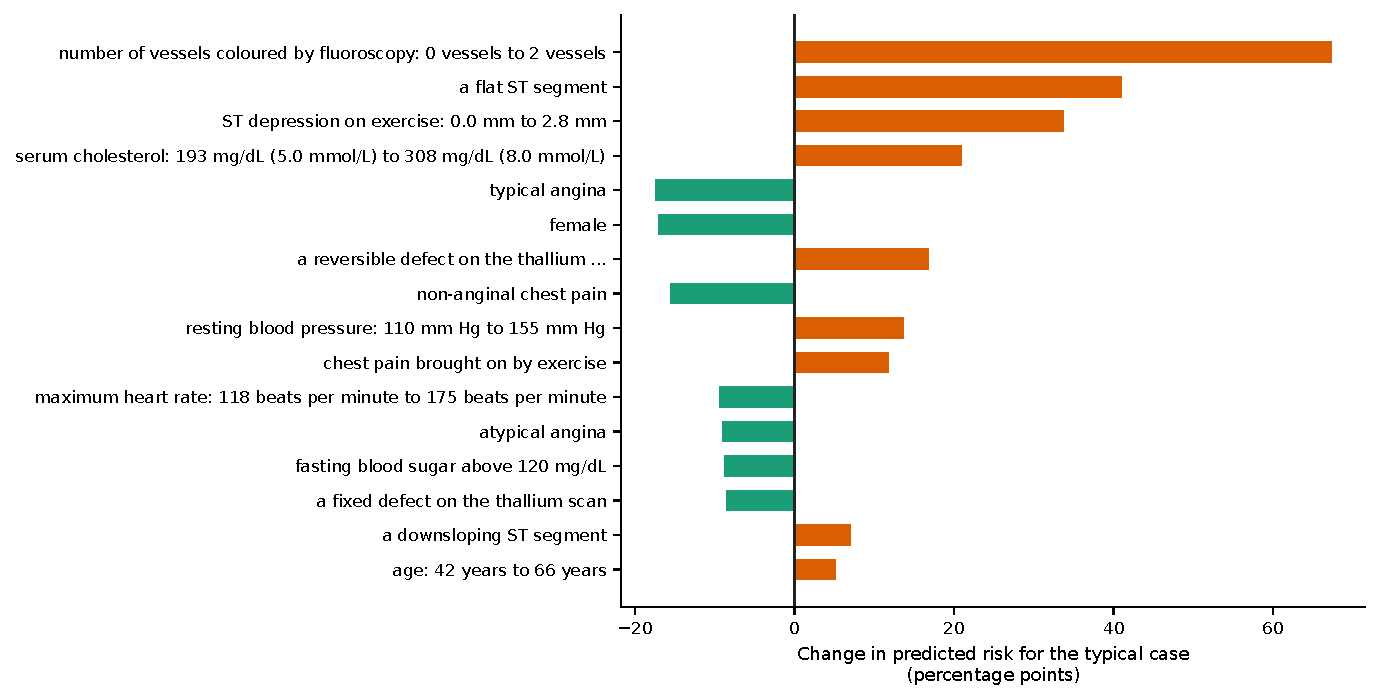
\includegraphics[width=\linewidth,height=0.88\textheight,keepaspectratio]{figures/heart-s5-c2/ann_38-effects.pdf}
\caption{The whole model: Each input's change in the predicted value for the typical case across the whole model, largest first (orange: raises it, teal: lowers it).}
\label{fig:hearts5c2:plot-ann38-0}
\end{figure}
\par\smallskip\noindent{\small \textbf{Dive deeper:} ST depression signal (\ref{rd:ann33}); Blood pressure step (\ref{rd:ann34}); Damping term (\ref{rd:ann35}); Hypertrophy without exercise pain (\ref{rd:ann36}); High fasting sugar term (\ref{rd:ann37}). Technical detail: \ref{tech:ann38}.\par}
\subsubsection{ST depression signal}\label{rd:ann33}
\noindent{\footnotesize Part of: The whole model (\ref{rd:ann38}).\par}
\noindent{\small Figure~\ref{fig:hearts5c2:parts-ann33} shows what feeds this part; Figure~\ref{fig:hearts5c2:units-ann33} its units and every connection into them (dashed boxes: connections from or to other parts, drawn in their own sections).\par}
\begin{figure}[H]\centering
\resizebox{!}{\ifdim\height>0.5\textheight 0.5\textheight\else\height\fi}{%
\resizebox{\ifdim\width>\linewidth\linewidth\else\width\fi}{!}{%
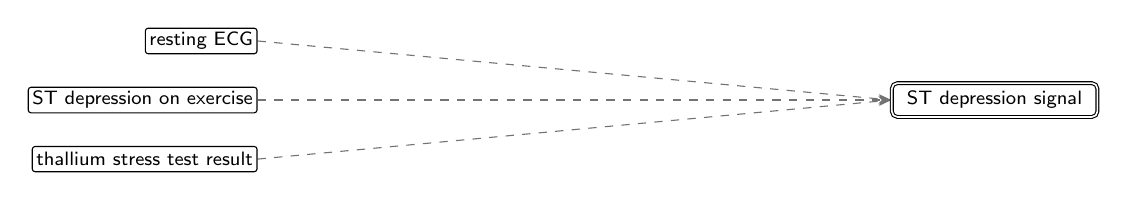
\begin{tikzpicture}[
  font=\sffamily\scriptsize, >={Stealth[length=1.6mm]},
  inp/.style={draw, rounded corners=1pt, fill=white, inner sep=1.5pt, minimum height=3.2mm, anchor=east},
  abox/.style={draw, thick, rounded corners=2pt, align=center, inner sep=3pt, minimum height=6mm, text width=42mm},
  outp/.style={draw, double, rounded corners=2pt, fill=white, align=center, inner sep=3pt, text width=24mm},
  agg/.style={draw=black!55},
]
\node[inp] (i0) at (0,0.75) {resting ECG};
\node[inp] (i1) at (0,-0.0) {ST depression on exercise};
\node[inp] (i2) at (0,-0.75) {thallium stress test result};
\node[outp] (out) at (9.36,0) {ST depression signal};
\begin{scope}[on background layer]
\draw[->, agg, thin, dashed] (i0.east) -- (out.west);
\draw[->, agg, thin, dashed] (i1.east) -- (out.west);
\draw[->, agg, thin, dashed] (i2.east) -- (out.west);
\end{scope}
\end{tikzpicture}}}%
\caption{ST depression signal: what feeds it, one level down.}
\label{fig:hearts5c2:parts-ann33}
\end{figure}
\begin{figure}[H]\centering
\resizebox{\ifdim\width>\linewidth\linewidth\else\width\fi}{!}{%
\definecolor{netup}{HTML}{D95F02}\definecolor{netdown}{HTML}{1B9E77}\definecolor{netmixed}{HTML}{7F7F7F}%
\begin{tikzpicture}[
  font=\sffamily\scriptsize, >={Stealth[length=1.4mm]},
  inp/.style={draw, circle, fill=white, minimum size=3.2mm, inner sep=0pt},
  hid/.style={draw, circle, fill=white, minimum size=5.2mm, inner sep=0.5pt, font=\sffamily\tiny},
  exitbox/.style={draw, thick, rectangle, fill=white, align=center, text width=17mm, minimum height=5mm, inner sep=1.5pt, font=\sffamily\tiny},
  sumbox/.style={draw, thick, dashed, rectangle, fill=white, align=center, text width=17mm, minimum height=5mm, inner sep=1.5pt, font=\sffamily\tiny},
  outp/.style={draw, thick, regular polygon, regular polygon sides=6, fill=white, minimum size=10mm, inner sep=0pt, font=\sffamily\tiny, align=center},
  stub/.style={draw, dashed, rounded corners=2pt, fill=white, align=center, inner sep=2pt, font=\sffamily\tiny, text width=15mm},
  inlab/.style={font=\sffamily\tiny, align=center, text width=15mm, inner sep=1pt, fill=white, fill opacity=0.8, text opacity=1},
  wpos/.style={draw=NavyBlue}, wneg/.style={draw=BrickRed}, wagg/.style={draw=black!45, line width=1.2pt},
  wmix/.style={draw=Plum},
]
\node[exitbox] (n204) at (2.7,1.9) {ST depression signal $\updownarrow$};
\node[inp, draw=netup, very thick] (ninxxoldpeak) at (0.9,0.0) {};
\path (ninxxoldpeak.south) node[inlab, anchor=north] (labninxxoldpeak) {ST depression $\uparrow$};
\node[inp, draw=netdown, very thick] (ninxxthalx4) at (4.5,0.0) {};
\path (ninxxthalx4.south) node[inlab, anchor=north] (labninxxthalx4) {thallium code 4 $\downarrow$};
\node[inp, draw=netup, very thick] (ninxxrestecgx0) at (2.7,0.0) {};
\path (ninxxrestecgx0.south) node[inlab, anchor=north] (labninxxrestecgx0) {normal ECG $\uparrow$};
\node[stub] (ntoxxthexmodelxoutput) at (-0.3,3.45) {to the model output};
\node[stub] (ntoxxBloodxpressurexstep) at (2.7,3.45) {to Blood pressure step};
\node[stub] (ntoxxDampingxterm) at (5.7,3.45) {to Damping term};
\begin{scope}[on background layer]
\node[fit=(n204) , inner sep=8pt, rounded corners=5pt, fill=BurntOrange!10, draw=BurntOrange!45] (clu0) {};
\draw[->, wpos, line width=1.14pt] (ninxxoldpeak) -- (n204);
\draw[->, wneg, line width=0.56pt] (ninxxthalx4) -- (n204);
\draw[->, wpos, line width=0.60pt] (ninxxrestecgx0) -- (n204);
\draw[->, wpos, line width=0.30pt] (n204) -- (ntoxxthexmodelxoutput);
\draw[->, wpos, line width=0.65pt] (n204) -- (ntoxxBloodxpressurexstep);
\draw[->, wpos, line width=0.54pt] (n204) -- (ntoxxDampingxterm);
\end{scope}
\node[font=\sffamily\scriptsize\bfseries, text=BurntOrange!55!black, anchor=south west, inner sep=1pt, fill=white, fill opacity=0.85, text opacity=1] at (clu0.north west) {ST depression signal};
\end{tikzpicture}}%
\caption{ST depression signal: its units and every connection into them. Blue: positive weight (raises the score); red: negative weight (lowers it); thicker: larger weight. Orange outline and up arrow: raises the final prediction; teal and down arrow: lowers it; grey and double arrow: depends.}
\label{fig:hearts5c2:units-ann33}
\end{figure}
\paragraph{Hypothesis.} This part raises the predicted risk with ST depression on exercise once it rises above about 1.3 mm, in an uneven way, and more so with a normal resting ECG.\,{\scriptsize\textcolor{NavyBlue}{[C35, C41, C39]}}
\paragraph{Evidence.} It acts on 109 of 242 training patients, 65 of whom had heart disease; for the typical patient it acts on, the predicted risk is about 76\% without it and about 89\% with it.\,{\scriptsize\textcolor{NavyBlue}{[C42]}} Through it, more ST depression adds to the risk only once it rises above about 1.3 mm (between 0.4 and 1.3 mm for different patients), rising in an uneven way: for a typical patient from about 16\% at 0 mm to about 50\% at 2.8 mm.\,{\scriptsize\textcolor{NavyBlue}{[C35, C41]}} ST depression counts more with a normal resting ECG (from about 16\% to about 50\%) than with any other resting ECG (from about 25\% to about 48\%), in an uneven way.\,{\scriptsize\textcolor{NavyBlue}{[C39]}} Through it, a resting ECG other than normal lowers a typical patient's risk from about 20\% to about 16\%, and a thallium result coded 4 shuts the signal (the model has little data on this, n = 2).\,{\scriptsize\textcolor{NavyBlue}{[C36, C37]}} Its formula reproduces the part exactly on all 242 training patients.\,{\scriptsize\textcolor{NavyBlue}{[C43]}}
\par\noindent{\small Evidence plots: Figure~\ref{fig:hearts5c2:plot-ann33-0}, Figure~\ref{fig:hearts5c2:plot-ann33-1}, Figure~\ref{fig:hearts5c2:plot-ann33-2}, Figure~\ref{fig:hearts5c2:plot-ann33-3}, Figure~\ref{fig:hearts5c2:plot-ann33-4}.\par}
\par\noindent{\small Figure~\ref{fig:hearts5c2:plot-ann33-3} shows this part's own output, unit h1: it switches on at about 0.3545 mm of ST depression on exercise, and is zero below.\par}
\begin{figure}[H]\centering
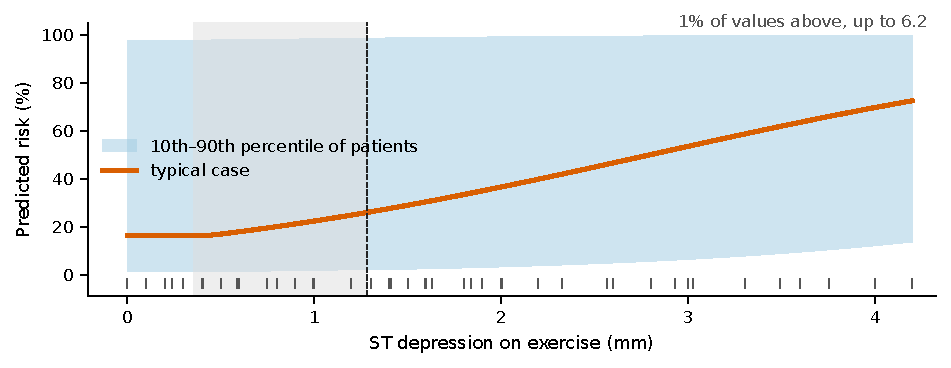
\includegraphics[width=\linewidth,height=0.88\textheight,keepaspectratio]{figures/heart-s5-c2/ann_33-response.pdf}
\caption{ST depression signal: Response curves through this part: the typical case (bold), the 10th to 90th percentile of individual patients (band), the fold or step point (dashed) with its spread across them (grey), and the observed values (ticks).}
\label{fig:hearts5c2:plot-ann33-0}
\end{figure}
\begin{figure}[H]\centering
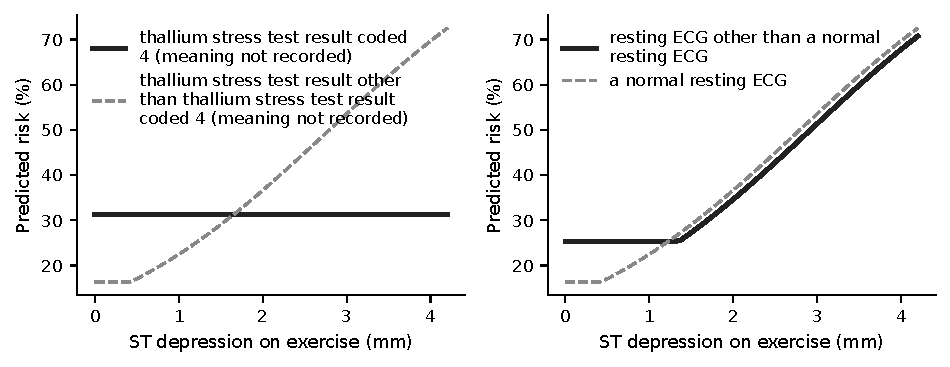
\includegraphics[width=\linewidth,height=0.88\textheight,keepaspectratio]{figures/heart-s5-c2/ann_33-interaction.pdf}
\caption{ST depression signal: How the effect differs between groups: one curve per group, for the typical case of each group.}
\label{fig:hearts5c2:plot-ann33-1}
\end{figure}
\begin{figure}[H]\centering
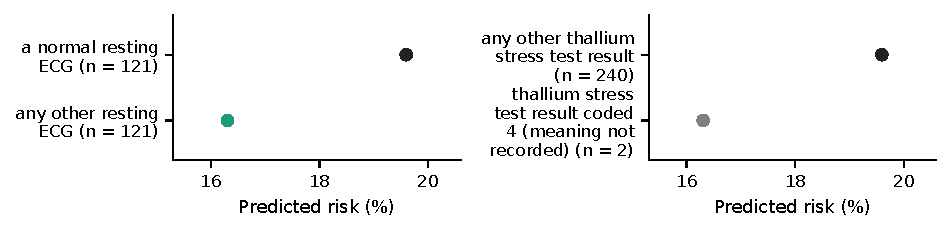
\includegraphics[width=\linewidth,height=0.88\textheight,keepaspectratio]{figures/heart-s5-c2/ann_33-categories-small.pdf}
\caption{ST depression signal: The predicted value for the typical case at each level, through this part (n = training patients; grey: fewer than 20).}
\label{fig:hearts5c2:plot-ann33-2}
\end{figure}
\begin{figure}[H]\centering
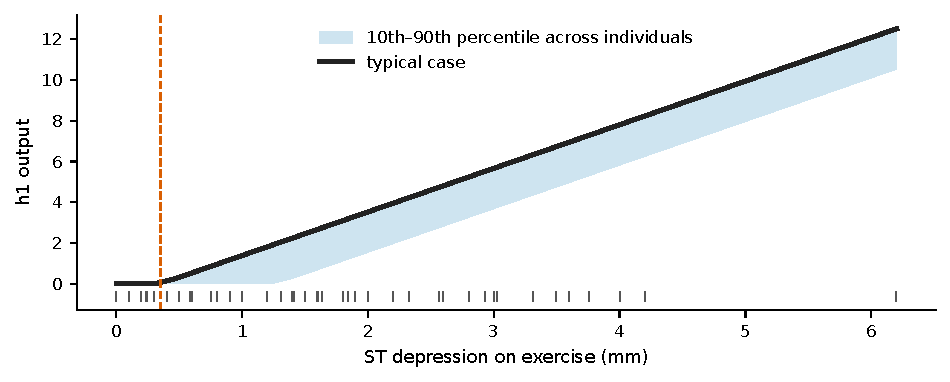
\includegraphics[width=\linewidth,height=0.88\textheight,keepaspectratio]{figures/heart-s5-c2/ann_33-partial-204.pdf}
\caption{ST depression signal: This part's own output, unit h1 (the output of 'ST depression signal'), on its own scale (its activation), with every other input at the typical case; it is active for 109 of 242. Bold: the typical case; band: 10th to 90th percentile across individuals; dashed: where it switches on; ticks: the data.}
\label{fig:hearts5c2:plot-ann33-3}
\end{figure}
\begin{figure}[H]\centering
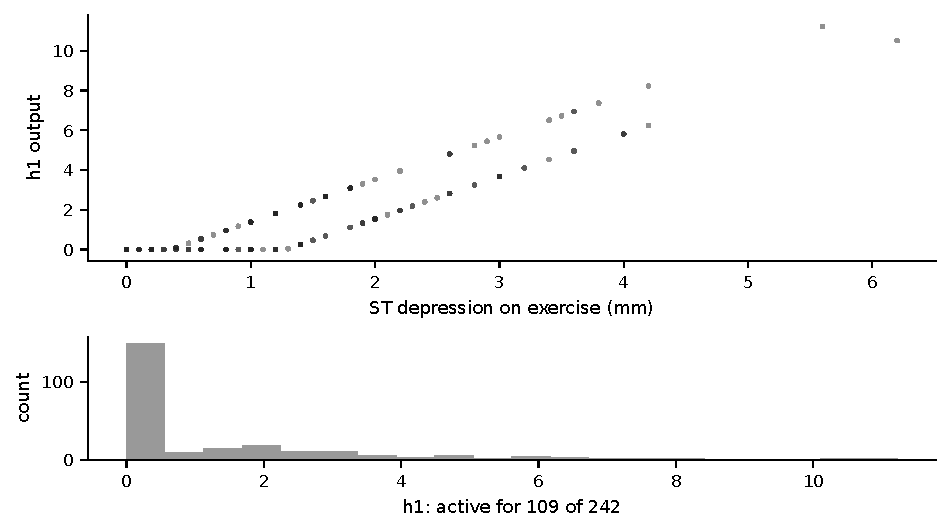
\includegraphics[width=\linewidth,height=0.88\textheight,keepaspectratio]{figures/heart-s5-c2/ann_33-units.pdf}
\caption{ST depression signal: This part's hidden units: each unit's output against its main numeric input (top) and how often it is active (bottom).}
\label{fig:hearts5c2:plot-ann33-4}
\end{figure}
\par\smallskip\noindent{\small Technical detail: \ref{tech:ann33}.\par}
\subsubsection{Blood pressure step}\label{rd:ann34}
\noindent{\footnotesize Part of: The whole model (\ref{rd:ann38}).\par}
\noindent{\small Figure~\ref{fig:hearts5c2:parts-ann34} shows what feeds this part; Figure~\ref{fig:hearts5c2:units-ann34} its units and every connection into them (dashed boxes: connections from or to other parts, drawn in their own sections).\par}
\begin{figure}[H]\centering
\resizebox{!}{\ifdim\height>0.5\textheight 0.5\textheight\else\height\fi}{%
\resizebox{\ifdim\width>\linewidth\linewidth\else\width\fi}{!}{%
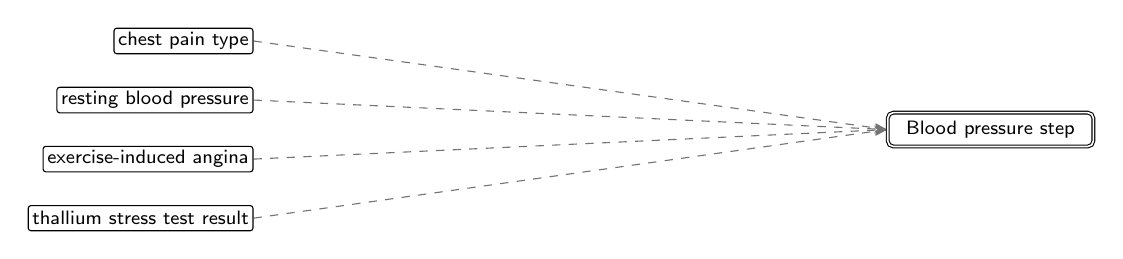
\begin{tikzpicture}[
  font=\sffamily\scriptsize, >={Stealth[length=1.6mm]},
  inp/.style={draw, rounded corners=1pt, fill=white, inner sep=1.5pt, minimum height=3.2mm, anchor=east},
  abox/.style={draw, thick, rounded corners=2pt, align=center, inner sep=3pt, minimum height=6mm, text width=42mm},
  outp/.style={draw, double, rounded corners=2pt, fill=white, align=center, inner sep=3pt, text width=24mm},
  agg/.style={draw=black!55},
]
\node[inp] (i0) at (0,1.125) {chest pain type};
\node[inp] (i1) at (0,0.375) {resting blood pressure};
\node[inp] (i2) at (0,-0.375) {exercise-induced angina};
\node[inp] (i3) at (0,-1.125) {thallium stress test result};
\node[outp] (out) at (9.36,0) {Blood pressure step};
\begin{scope}[on background layer]
\draw[->, agg, thin, dashed] (i0.east) -- (out.west);
\draw[->, agg, thin, dashed] (i1.east) -- (out.west);
\draw[->, agg, thin, dashed] (i2.east) -- (out.west);
\draw[->, agg, thin, dashed] (i3.east) -- (out.west);
\end{scope}
\end{tikzpicture}}}%
\caption{Blood pressure step: what feeds it, one level down.}
\label{fig:hearts5c2:parts-ann34}
\end{figure}
\begin{figure}[H]\centering
\resizebox{\ifdim\width>\linewidth\linewidth\else\width\fi}{!}{%
\definecolor{netup}{HTML}{D95F02}\definecolor{netdown}{HTML}{1B9E77}\definecolor{netmixed}{HTML}{7F7F7F}%
\begin{tikzpicture}[
  font=\sffamily\scriptsize, >={Stealth[length=1.4mm]},
  inp/.style={draw, circle, fill=white, minimum size=3.2mm, inner sep=0pt},
  hid/.style={draw, circle, fill=white, minimum size=5.2mm, inner sep=0.5pt, font=\sffamily\tiny},
  exitbox/.style={draw, thick, rectangle, fill=white, align=center, text width=17mm, minimum height=5mm, inner sep=1.5pt, font=\sffamily\tiny},
  sumbox/.style={draw, thick, dashed, rectangle, fill=white, align=center, text width=17mm, minimum height=5mm, inner sep=1.5pt, font=\sffamily\tiny},
  outp/.style={draw, thick, regular polygon, regular polygon sides=6, fill=white, minimum size=10mm, inner sep=0pt, font=\sffamily\tiny, align=center},
  stub/.style={draw, dashed, rounded corners=2pt, fill=white, align=center, inner sep=2pt, font=\sffamily\tiny, text width=15mm},
  inlab/.style={font=\sffamily\tiny, align=center, text width=15mm, inner sep=1pt, fill=white, fill opacity=0.8, text opacity=1},
  wpos/.style={draw=NavyBlue}, wneg/.style={draw=BrickRed}, wagg/.style={draw=black!45, line width=1.2pt},
  wmix/.style={draw=Plum},
]
\node[exitbox] (n290) at (4.5,3.25) {Blood pressure step $\uparrow$};
\node[hid] (nidentityx290) at (4.5,1.9) {h6};
\node[inp, draw=netdown, very thick] (ninxxexangx1) at (2.7,0.0) {};
\path (ninxxexangx1.south) node[inlab, anchor=north] (labninxxexangx1) {exercise pain $\downarrow$};
\node[inp, draw=netdown, very thick] (ninxxthalx6) at (4.5,0.0) {};
\path (ninxxthalx6.south) node[inlab, anchor=north] (labninxxthalx6) {fixed defect $\downarrow$};
\node[inp, draw=netdown, very thick] (ninxxtrestbps) at (0.9,0.0) {};
\path (ninxxtrestbps.south) node[inlab, anchor=north] (labninxxtrestbps) {blood pressure $\downarrow$};
\node[inp, draw=netdown, very thick] (ninxxcpx3) at (8.1,0.0) {};
\path (ninxxcpx3.south) node[inlab, anchor=north] (labninxxcpx3) {non-anginal pain $\downarrow$};
\node[stub] (nfromxxSTxdepressionxsignal) at (6.3,0.0) {from ST depression signal};
\node[stub] (ntoxxthexmodelxoutput) at (4.5,4.8) {to the model output};
\begin{scope}[on background layer]
\node[fit=(n290) (nidentityx290) , inner sep=8pt, rounded corners=5pt, fill=ForestGreen!10, draw=ForestGreen!45] (clu0) {};
\draw[->, wneg, line width=0.30pt] (ninxxexangx1) -- (n290);
\draw[->, wneg, line width=0.25pt] (ninxxthalx6) -- (n290);
\draw[->, wneg, line width=0.52pt] (ninxxtrestbps) -- (n290);
\draw[->, wneg, line width=0.27pt] (ninxxcpx3) -- (n290);
\draw[->, wpos, line width=0.65pt] (nfromxxSTxdepressionxsignal) -- (nidentityx290);
\draw[->, wpos, line width=0.60pt] (nidentityx290) -- (n290);
\draw[->, wpos, line width=0.34pt] (n290) -- (ntoxxthexmodelxoutput);
\end{scope}
\node[font=\sffamily\scriptsize\bfseries, text=ForestGreen!55!black, anchor=south west, inner sep=1pt, fill=white, fill opacity=0.85, text opacity=1] at (clu0.north west) {Blood pressure step};
\end{tikzpicture}}%
\caption{Blood pressure step: its units and every connection into them. Blue: positive weight (raises the score); red: negative weight (lowers it); thicker: larger weight. Orange outline and up arrow: raises the final prediction; teal and down arrow: lowers it; grey and double arrow: depends.}
\label{fig:hearts5c2:units-ann34}
\end{figure}
\paragraph{Hypothesis.} This part passes the ST depression signal on to the predicted risk, more for patients with lower resting blood pressure: through it, higher resting blood pressure lowers the risk in an uneven way up to about 125 mm Hg (between 122 mm Hg and 165 mm Hg for different patients), then no further.\,{\scriptsize\textcolor{NavyBlue}{[C53, C44, C52]}}
\paragraph{Evidence.} It acts on 145 of 242 training patients, 73 of whom had heart disease; for the typical patient it acts on, the predicted risk is about 51\% without it and about 68\% with it.\,{\scriptsize\textcolor{NavyBlue}{[C53]}} Through it, higher resting blood pressure lowers the risk up to about 125 mm Hg (between 122 and 165 mm Hg for different patients), then no further, in an uneven way: for a typical patient from about 23\% at 110 mm Hg to about 17\% at 155 mm Hg.\,{\scriptsize\textcolor{NavyBlue}{[C44, C52]}} Through it, chest pain on exercise lowers a typical patient's risk from about 20\% to about 18\%, and non-anginal chest pain to about 19\%.\,{\scriptsize\textcolor{NavyBlue}{[C45, C46]}} Its formula reproduces the part exactly on all 242 training patients.\,{\scriptsize\textcolor{NavyBlue}{[C54]}}
\par\noindent{\small Evidence plots: Figure~\ref{fig:hearts5c2:plot-ann34-0}, Figure~\ref{fig:hearts5c2:plot-ann34-1}, Figure~\ref{fig:hearts5c2:plot-ann34-2}, Figure~\ref{fig:hearts5c2:plot-ann34-3}.\par}
\par\noindent{\small Figure~\ref{fig:hearts5c2:plot-ann34-2} shows this part's own output, unit h2: over its two main inputs, with the line where it switches on.\par}
\begin{figure}[H]\centering
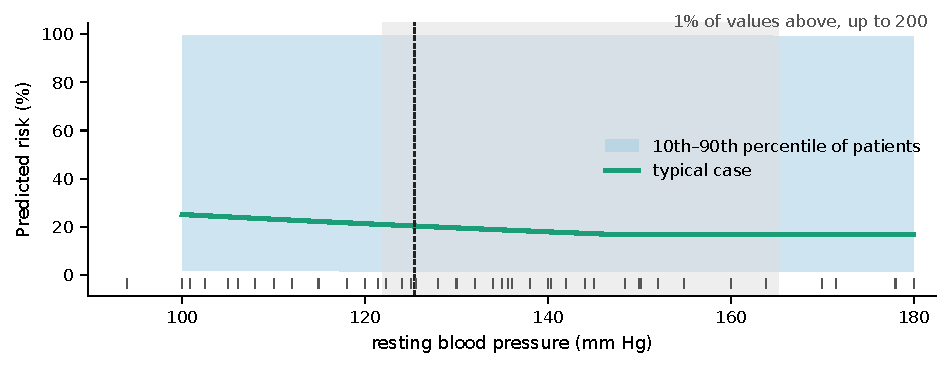
\includegraphics[width=\linewidth,height=0.88\textheight,keepaspectratio]{figures/heart-s5-c2/ann_34-response.pdf}
\caption{Blood pressure step: Response curves through this part: the typical case (bold), the 10th to 90th percentile of individual patients (band), the fold or step point (dashed) with its spread across them (grey), and the observed values (ticks).}
\label{fig:hearts5c2:plot-ann34-0}
\end{figure}
\begin{figure}[H]\centering
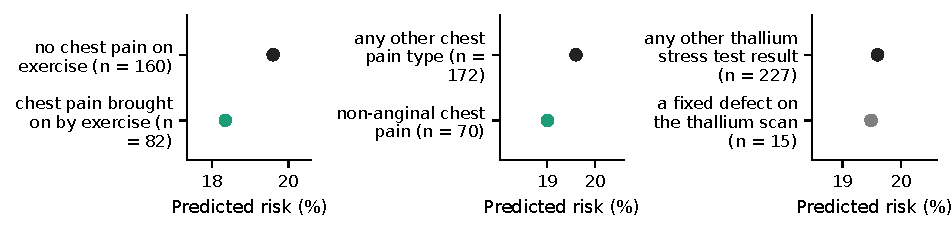
\includegraphics[width=\linewidth,height=0.88\textheight,keepaspectratio]{figures/heart-s5-c2/ann_34-categories-small.pdf}
\caption{Blood pressure step: The predicted value for the typical case at each level, through this part (n = training patients; grey: fewer than 20).}
\label{fig:hearts5c2:plot-ann34-1}
\end{figure}
\begin{figure}[H]\centering
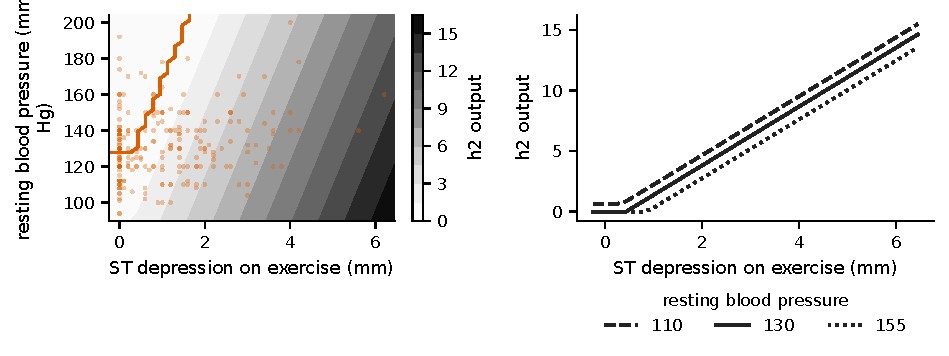
\includegraphics[width=\linewidth,height=0.88\textheight,keepaspectratio]{figures/heart-s5-c2/ann_34-partial-290.pdf}
\caption{Blood pressure step: This part's own output, unit h2 (the output of 'Blood pressure step'), on its own scale (its activation), with every other input at the typical case; it is active for 145 of 242. Left: its output over its two main inputs (orange line: where it switches on; dots: the data); right: slices at three values of the second input.}
\label{fig:hearts5c2:plot-ann34-2}
\end{figure}
\begin{figure}[H]\centering
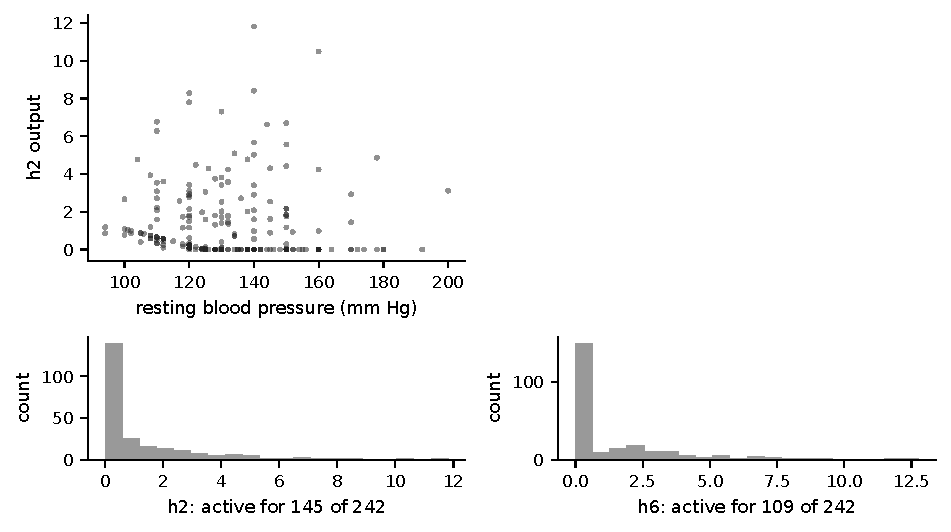
\includegraphics[width=\linewidth,height=0.88\textheight,keepaspectratio]{figures/heart-s5-c2/ann_34-units.pdf}
\caption{Blood pressure step: This part's hidden units: each unit's output against its main numeric input (top) and how often it is active (bottom).}
\label{fig:hearts5c2:plot-ann34-3}
\end{figure}
\par\smallskip\noindent{\small Technical detail: \ref{tech:ann34}.\par}
\subsubsection{Damping term}\label{rd:ann35}
\noindent{\footnotesize Part of: The whole model (\ref{rd:ann38}).\par}
\noindent{\small Figure~\ref{fig:hearts5c2:parts-ann35} shows what feeds this part; Figure~\ref{fig:hearts5c2:units-ann35} its units and every connection into them (dashed boxes: connections from or to other parts, drawn in their own sections).\par}
\begin{figure}[H]\centering
\resizebox{!}{\ifdim\height>0.5\textheight 0.5\textheight\else\height\fi}{%
\resizebox{\ifdim\width>\linewidth\linewidth\else\width\fi}{!}{%
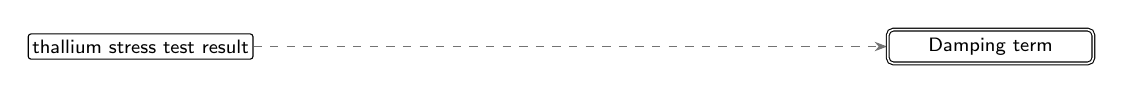
\begin{tikzpicture}[
  font=\sffamily\scriptsize, >={Stealth[length=1.6mm]},
  inp/.style={draw, rounded corners=1pt, fill=white, inner sep=1.5pt, minimum height=3.2mm, anchor=east},
  abox/.style={draw, thick, rounded corners=2pt, align=center, inner sep=3pt, minimum height=6mm, text width=42mm},
  outp/.style={draw, double, rounded corners=2pt, fill=white, align=center, inner sep=3pt, text width=24mm},
  agg/.style={draw=black!55},
]
\node[inp] (i0) at (0,-0.0) {thallium stress test result};
\node[outp] (out) at (9.36,0) {Damping term};
\begin{scope}[on background layer]
\draw[->, agg, thin, dashed] (i0.east) -- (out.west);
\end{scope}
\end{tikzpicture}}}%
\caption{Damping term: what feeds it, one level down.}
\label{fig:hearts5c2:parts-ann35}
\end{figure}
\begin{figure}[H]\centering
\resizebox{\ifdim\width>\linewidth\linewidth\else\width\fi}{!}{%
\definecolor{netup}{HTML}{D95F02}\definecolor{netdown}{HTML}{1B9E77}\definecolor{netmixed}{HTML}{7F7F7F}%
\begin{tikzpicture}[
  font=\sffamily\scriptsize, >={Stealth[length=1.4mm]},
  inp/.style={draw, circle, fill=white, minimum size=3.2mm, inner sep=0pt},
  hid/.style={draw, circle, fill=white, minimum size=5.2mm, inner sep=0.5pt, font=\sffamily\tiny},
  exitbox/.style={draw, thick, rectangle, fill=white, align=center, text width=17mm, minimum height=5mm, inner sep=1.5pt, font=\sffamily\tiny},
  sumbox/.style={draw, thick, dashed, rectangle, fill=white, align=center, text width=17mm, minimum height=5mm, inner sep=1.5pt, font=\sffamily\tiny},
  outp/.style={draw, thick, regular polygon, regular polygon sides=6, fill=white, minimum size=10mm, inner sep=0pt, font=\sffamily\tiny, align=center},
  stub/.style={draw, dashed, rounded corners=2pt, fill=white, align=center, inner sep=2pt, font=\sffamily\tiny, text width=15mm},
  inlab/.style={font=\sffamily\tiny, align=center, text width=15mm, inner sep=1pt, fill=white, fill opacity=0.8, text opacity=1},
  wpos/.style={draw=NavyBlue}, wneg/.style={draw=BrickRed}, wagg/.style={draw=black!45, line width=1.2pt},
  wmix/.style={draw=Plum},
]
\node[hid] (nidentityx1416) at (1.8,1.9) {h7};
\node[exitbox] (n1416) at (1.8,3.25) {Damping term $\downarrow$};
\node[inp, draw=netup, very thick] (ninxxthalx6) at (0.9,0.0) {};
\path (ninxxthalx6.south) node[inlab, anchor=north] (labninxxthalx6) {fixed defect $\uparrow$};
\node[stub] (nfromxxSTxdepressionxsignal) at (2.7,0.0) {from ST depression signal};
\node[stub] (ntoxxthexmodelxoutput) at (1.8,4.8) {to the model output};
\begin{scope}[on background layer]
\node[fit=(nidentityx1416) (n1416) , inner sep=8pt, rounded corners=5pt, fill=Orchid!10, draw=Orchid!45] (clu0) {};
\draw[->, wneg, line width=0.46pt] (ninxxthalx6) -- (n1416);
\draw[->, wpos, line width=0.54pt] (nfromxxSTxdepressionxsignal) -- (nidentityx1416);
\draw[->, wpos, line width=0.60pt] (nidentityx1416) -- (n1416);
\draw[->, wneg, line width=0.29pt] (n1416) -- (ntoxxthexmodelxoutput);
\end{scope}
\node[font=\sffamily\scriptsize\bfseries, text=Orchid!55!black, anchor=south west, inner sep=1pt, fill=white, fill opacity=0.85, text opacity=1] at (clu0.north west) {Damping term};
\end{tikzpicture}}%
\caption{Damping term: its units and every connection into them. Blue: positive weight (raises the score); red: negative weight (lowers it); thicker: larger weight. Orange outline and up arrow: raises the final prediction; teal and down arrow: lowers it; grey and double arrow: depends.}
\label{fig:hearts5c2:units-ann35}
\end{figure}
\paragraph{Hypothesis.} This part takes back a little of the ST depression signal for nearly every patient and adds a little for a fixed defect on the thallium scan (the model has little data on this, n = 15).\,{\scriptsize\textcolor{NavyBlue}{[C56, C55]}}
\paragraph{Evidence.} It acts on 234 of 242 training patients, 102 of whom had heart disease; for the typical patient it acts on, the predicted risk is about 24\% without it and about 20\% with it.\,{\scriptsize\textcolor{NavyBlue}{[C56]}} Through it, a fixed defect on the thallium scan raises a typical patient's risk from about 20\% to about 23\% (the model has little data on this, n = 15).\,{\scriptsize\textcolor{NavyBlue}{[C55]}} Its formula reproduces the part exactly on all 242 training patients.\,{\scriptsize\textcolor{NavyBlue}{[C57]}}
\par\noindent{\small Evidence plots: Figure~\ref{fig:hearts5c2:plot-ann35-0}, Figure~\ref{fig:hearts5c2:plot-ann35-1}, Figure~\ref{fig:hearts5c2:plot-ann35-2}.\par}
\par\noindent{\small Figure~\ref{fig:hearts5c2:plot-ann35-1} shows this part's own output, unit h3.\par}
\begin{figure}[H]\centering
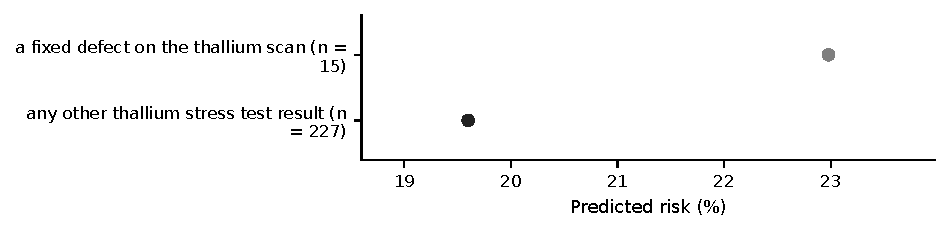
\includegraphics[width=\linewidth,height=0.88\textheight,keepaspectratio]{figures/heart-s5-c2/ann_35-categories-small.pdf}
\caption{Damping term: The predicted value for the typical case at each level, through this part (n = training patients; grey: fewer than 20).}
\label{fig:hearts5c2:plot-ann35-0}
\end{figure}
\begin{figure}[H]\centering
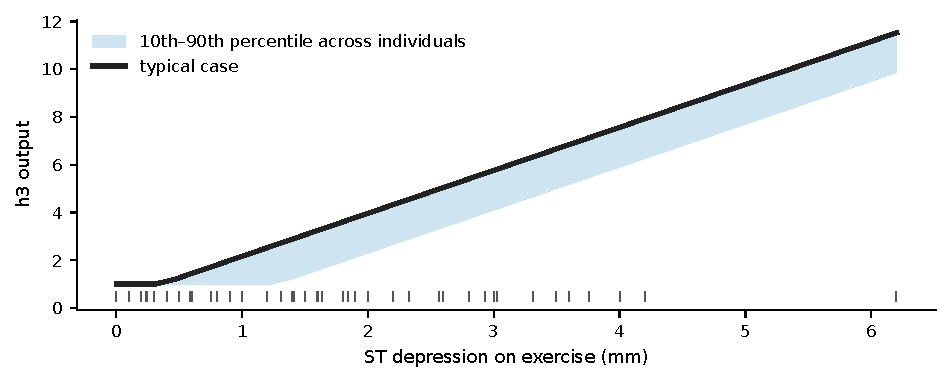
\includegraphics[width=\linewidth,height=0.88\textheight,keepaspectratio]{figures/heart-s5-c2/ann_35-partial-1416.pdf}
\caption{Damping term: This part's own output, unit h3 (the output of 'Damping term'), on its own scale (its activation), with every other input at the typical case; it is active for 234 of 242. Bold: the typical case; band: 10th to 90th percentile across individuals; ticks: the data.}
\label{fig:hearts5c2:plot-ann35-1}
\end{figure}
\begin{figure}[H]\centering
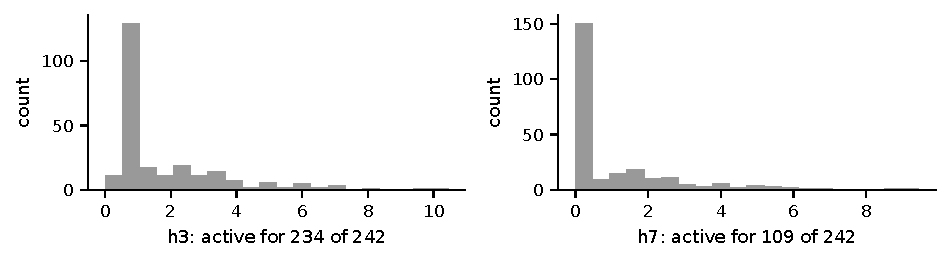
\includegraphics[width=\linewidth,height=0.88\textheight,keepaspectratio]{figures/heart-s5-c2/ann_35-units.pdf}
\caption{Damping term: This part's hidden units: each unit's output against its main numeric input (top) and how often it is active (bottom).}
\label{fig:hearts5c2:plot-ann35-2}
\end{figure}
\par\smallskip\noindent{\small Technical detail: \ref{tech:ann35}.\par}
\subsubsection{Hypertrophy without exercise pain}\label{rd:ann36}
\noindent{\footnotesize Part of: The whole model (\ref{rd:ann38}).\par}
\noindent{\small Figure~\ref{fig:hearts5c2:parts-ann36} shows what feeds this part; Figure~\ref{fig:hearts5c2:units-ann36} its units and every connection into them (dashed boxes: connections from or to other parts, drawn in their own sections).\par}
\begin{figure}[H]\centering
\resizebox{!}{\ifdim\height>0.5\textheight 0.5\textheight\else\height\fi}{%
\resizebox{\ifdim\width>\linewidth\linewidth\else\width\fi}{!}{%
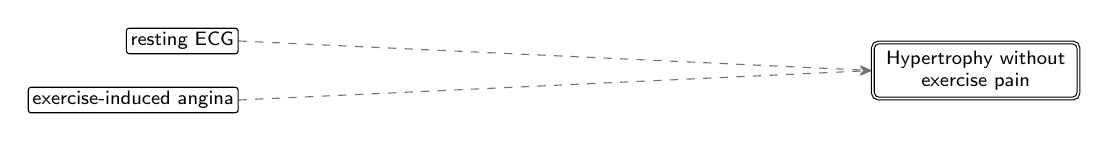
\begin{tikzpicture}[
  font=\sffamily\scriptsize, >={Stealth[length=1.6mm]},
  inp/.style={draw, rounded corners=1pt, fill=white, inner sep=1.5pt, minimum height=3.2mm, anchor=east},
  abox/.style={draw, thick, rounded corners=2pt, align=center, inner sep=3pt, minimum height=6mm, text width=42mm},
  outp/.style={draw, double, rounded corners=2pt, fill=white, align=center, inner sep=3pt, text width=24mm},
  agg/.style={draw=black!55},
]
\node[inp] (i0) at (0,0.375) {resting ECG};
\node[inp] (i1) at (0,-0.375) {exercise-induced angina};
\node[outp] (out) at (9.36,0) {Hypertrophy without exercise pain};
\begin{scope}[on background layer]
\draw[->, agg, thin, dashed] (i0.east) -- (out.west);
\draw[->, agg, thin, dashed] (i1.east) -- (out.west);
\end{scope}
\end{tikzpicture}}}%
\caption{Hypertrophy without exercise pain: what feeds it, one level down.}
\label{fig:hearts5c2:parts-ann36}
\end{figure}
\begin{figure}[H]\centering
\resizebox{\ifdim\width>\linewidth\linewidth\else\width\fi}{!}{%
\definecolor{netup}{HTML}{D95F02}\definecolor{netdown}{HTML}{1B9E77}\definecolor{netmixed}{HTML}{7F7F7F}%
\begin{tikzpicture}[
  font=\sffamily\scriptsize, >={Stealth[length=1.4mm]},
  inp/.style={draw, circle, fill=white, minimum size=3.2mm, inner sep=0pt},
  hid/.style={draw, circle, fill=white, minimum size=5.2mm, inner sep=0.5pt, font=\sffamily\tiny},
  exitbox/.style={draw, thick, rectangle, fill=white, align=center, text width=17mm, minimum height=5mm, inner sep=1.5pt, font=\sffamily\tiny},
  sumbox/.style={draw, thick, dashed, rectangle, fill=white, align=center, text width=17mm, minimum height=5mm, inner sep=1.5pt, font=\sffamily\tiny},
  outp/.style={draw, thick, regular polygon, regular polygon sides=6, fill=white, minimum size=10mm, inner sep=0pt, font=\sffamily\tiny, align=center},
  stub/.style={draw, dashed, rounded corners=2pt, fill=white, align=center, inner sep=2pt, font=\sffamily\tiny, text width=15mm},
  inlab/.style={font=\sffamily\tiny, align=center, text width=15mm, inner sep=1pt, fill=white, fill opacity=0.8, text opacity=1},
  wpos/.style={draw=NavyBlue}, wneg/.style={draw=BrickRed}, wagg/.style={draw=black!45, line width=1.2pt},
  wmix/.style={draw=Plum},
]
\node[exitbox] (n1611) at (3.3,1.9) {Hypertrophy without exercise pain $\uparrow$};
\node[inp, draw=netup, very thick] (ninxxrestecgx2) at (2.4,0.0) {};
\path (ninxxrestecgx2.south) node[inlab, anchor=north] (labninxxrestecgx2) {LVH on ECG $\uparrow$};
\node[inp, draw=netdown, very thick] (ninxxexangx1) at (4.2,0.0) {};
\path (ninxxexangx1.south) node[inlab, anchor=north] (labninxxexangx1) {exercise pain $\downarrow$};
\node[stub] (ntoxxthexmodelxoutput) at (3.3,3.45) {to the model output};
\begin{scope}[on background layer]
\node[fit=(n1611) , inner sep=8pt, rounded corners=5pt, fill=Goldenrod!10, draw=Goldenrod!45] (clu0) {};
\draw[->, wpos, line width=0.56pt] (ninxxrestecgx2) -- (n1611);
\draw[->, wneg, line width=0.58pt] (ninxxexangx1) -- (n1611);
\draw[->, wpos, line width=0.51pt] (n1611) -- (ntoxxthexmodelxoutput);
\end{scope}
\node[font=\sffamily\scriptsize\bfseries, text=Goldenrod!55!black, anchor=south west, inner sep=1pt, fill=white, fill opacity=0.85, text opacity=1] at (clu0.north west) {Hypertrophy without exercise pain};
\end{tikzpicture}}%
\caption{Hypertrophy without exercise pain: its units and every connection into them. Blue: positive weight (raises the score); red: negative weight (lowers it); thicker: larger weight. Orange outline and up arrow: raises the final prediction; teal and down arrow: lowers it; grey and double arrow: depends.}
\label{fig:hearts5c2:units-ann36}
\end{figure}
\paragraph{Hypothesis.} This part adds a little to the predicted risk for patients with left ventricular hypertrophy on the resting ECG and no chest pain on exercise.\,{\scriptsize\textcolor{NavyBlue}{[C61, C59]}}
\paragraph{Evidence.} It acts on 74 of 242 training patients, nearly all with left ventricular hypertrophy and no chest pain on exercise, 30 of whom had heart disease; for the typical patient it acts on, the predicted risk is about 25\% without it and about 30\% with it.\,{\scriptsize\textcolor{NavyBlue}{[C61]}} Through it, left ventricular hypertrophy raises a typical patient's risk from about 20\% to about 24\%, and for the typical patient it acts on, chest pain on exercise lowers it from about 30\% to about 25\%.\,{\scriptsize\textcolor{NavyBlue}{[C59, C58]}} Across the model, chest pain on exercise raises a typical patient's risk from about 20\% to about 31\% without left ventricular hypertrophy, and from about 25\% to about 35\% with it.\,{\scriptsize\textcolor{NavyBlue}{[C60]}} Its formula reproduces the part exactly on all 242 training patients.\,{\scriptsize\textcolor{NavyBlue}{[C63]}}
\par\noindent{\small Evidence plots: Figure~\ref{fig:hearts5c2:plot-ann36-0}, Figure~\ref{fig:hearts5c2:plot-ann36-1}, Figure~\ref{fig:hearts5c2:plot-ann36-2}.\par}
\par\noindent{\small Figure~\ref{fig:hearts5c2:plot-ann36-1} shows this part's own output, unit h4.\par}
\begin{figure}[H]\centering
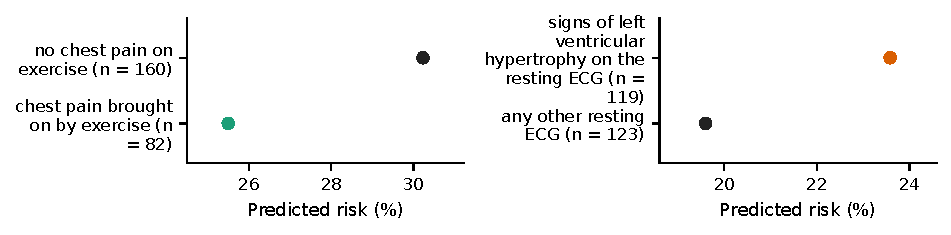
\includegraphics[width=\linewidth,height=0.88\textheight,keepaspectratio]{figures/heart-s5-c2/ann_36-categories-small.pdf}
\caption{Hypertrophy without exercise pain: The predicted value for the typical case at each level, through this part (n = training patients; grey: fewer than 20).}
\label{fig:hearts5c2:plot-ann36-0}
\end{figure}
\begin{figure}[H]\centering
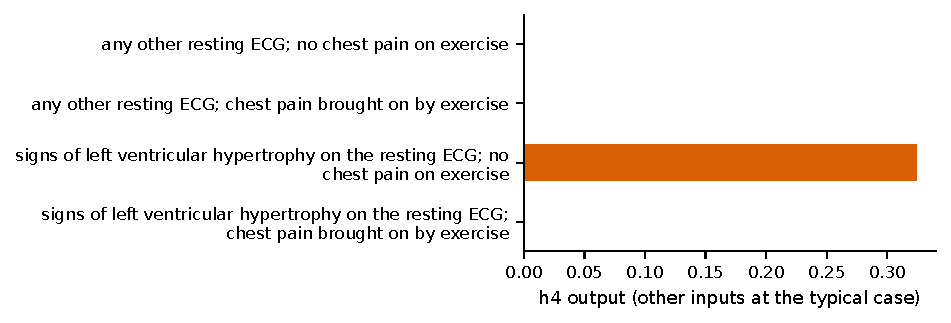
\includegraphics[width=\linewidth,height=0.88\textheight,keepaspectratio]{figures/heart-s5-c2/ann_36-partial-1611.pdf}
\caption{Hypertrophy without exercise pain: This part's own output, unit h4 (the output of 'Hypertrophy without exercise pain'), on its own scale (its activation), with every other input at the typical case; it is active for 74 of 242. Its output for each combination of the levels it reads.}
\label{fig:hearts5c2:plot-ann36-1}
\end{figure}
\begin{figure}[H]\centering
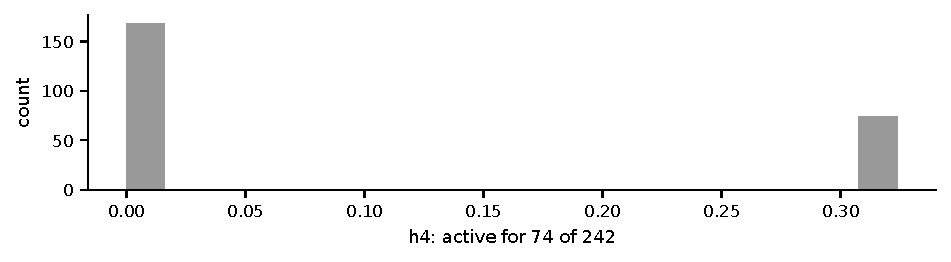
\includegraphics[width=\linewidth,height=0.88\textheight,keepaspectratio]{figures/heart-s5-c2/ann_36-units.pdf}
\caption{Hypertrophy without exercise pain: This part's hidden units: each unit's output against its main numeric input (top) and how often it is active (bottom).}
\label{fig:hearts5c2:plot-ann36-2}
\end{figure}
\par\smallskip\noindent{\small Technical detail: \ref{tech:ann36}.\par}
\subsubsection{High fasting sugar term}\label{rd:ann37}
\noindent{\footnotesize Part of: The whole model (\ref{rd:ann38}).\par}
\noindent{\small Figure~\ref{fig:hearts5c2:parts-ann37} shows what feeds this part; Figure~\ref{fig:hearts5c2:units-ann37} its units and every connection into them (dashed boxes: connections from or to other parts, drawn in their own sections).\par}
\begin{figure}[H]\centering
\resizebox{!}{\ifdim\height>0.5\textheight 0.5\textheight\else\height\fi}{%
\resizebox{\ifdim\width>\linewidth\linewidth\else\width\fi}{!}{%
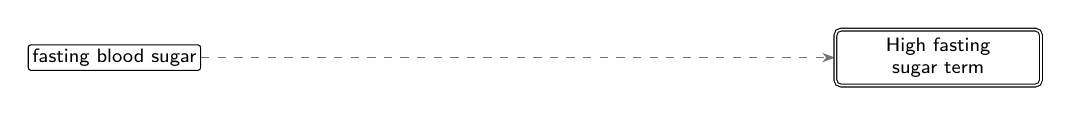
\begin{tikzpicture}[
  font=\sffamily\scriptsize, >={Stealth[length=1.6mm]},
  inp/.style={draw, rounded corners=1pt, fill=white, inner sep=1.5pt, minimum height=3.2mm, anchor=east},
  abox/.style={draw, thick, rounded corners=2pt, align=center, inner sep=3pt, minimum height=6mm, text width=42mm},
  outp/.style={draw, double, rounded corners=2pt, fill=white, align=center, inner sep=3pt, text width=24mm},
  agg/.style={draw=black!55},
]
\node[inp] (i0) at (0,-0.0) {fasting blood sugar};
\node[outp] (out) at (9.36,0) {High fasting sugar term};
\begin{scope}[on background layer]
\draw[->, agg, thin, dashed] (i0.east) -- (out.west);
\end{scope}
\end{tikzpicture}}}%
\caption{High fasting sugar term: what feeds it, one level down.}
\label{fig:hearts5c2:parts-ann37}
\end{figure}
\begin{figure}[H]\centering
\resizebox{\ifdim\width>\linewidth\linewidth\else\width\fi}{!}{%
\definecolor{netup}{HTML}{D95F02}\definecolor{netdown}{HTML}{1B9E77}\definecolor{netmixed}{HTML}{7F7F7F}%
\begin{tikzpicture}[
  font=\sffamily\scriptsize, >={Stealth[length=1.4mm]},
  inp/.style={draw, circle, fill=white, minimum size=3.2mm, inner sep=0pt},
  hid/.style={draw, circle, fill=white, minimum size=5.2mm, inner sep=0.5pt, font=\sffamily\tiny},
  exitbox/.style={draw, thick, rectangle, fill=white, align=center, text width=17mm, minimum height=5mm, inner sep=1.5pt, font=\sffamily\tiny},
  sumbox/.style={draw, thick, dashed, rectangle, fill=white, align=center, text width=17mm, minimum height=5mm, inner sep=1.5pt, font=\sffamily\tiny},
  outp/.style={draw, thick, regular polygon, regular polygon sides=6, fill=white, minimum size=10mm, inner sep=0pt, font=\sffamily\tiny, align=center},
  stub/.style={draw, dashed, rounded corners=2pt, fill=white, align=center, inner sep=2pt, font=\sffamily\tiny, text width=15mm},
  inlab/.style={font=\sffamily\tiny, align=center, text width=15mm, inner sep=1pt, fill=white, fill opacity=0.8, text opacity=1},
  wpos/.style={draw=NavyBlue}, wneg/.style={draw=BrickRed}, wagg/.style={draw=black!45, line width=1.2pt},
  wmix/.style={draw=Plum},
]
\node[exitbox] (n3884) at (2.3,1.9) {High fasting sugar term $\uparrow$};
\node[inp, draw=netup, very thick] (ninxxfbsx1) at (2.3,0.0) {};
\path (ninxxfbsx1.south) node[inlab, anchor=north] (labninxxfbsx1) {sugar above 120 $\uparrow$};
\node[stub] (ntoxxthexmodelxoutput) at (2.3,3.45) {to the model output};
\begin{scope}[on background layer]
\node[fit=(n3884) , inner sep=8pt, rounded corners=5pt, fill=Cerulean!10, draw=Cerulean!45] (clu0) {};
\draw[->, wpos, line width=0.60pt] (ninxxfbsx1) -- (n3884);
\draw[->, wpos, line width=0.27pt] (n3884) -- (ntoxxthexmodelxoutput);
\end{scope}
\node[font=\sffamily\scriptsize\bfseries, text=Cerulean!55!black, anchor=south west, inner sep=1pt, fill=white, fill opacity=0.85, text opacity=1] at (clu0.north west) {High fasting sugar term};
\end{tikzpicture}}%
\caption{High fasting sugar term: its units and every connection into them. Blue: positive weight (raises the score); red: negative weight (lowers it); thicker: larger weight. Orange outline and up arrow: raises the final prediction; teal and down arrow: lowers it; grey and double arrow: depends.}
\label{fig:hearts5c2:units-ann37}
\end{figure}
\paragraph{Hypothesis.} This part adds a very small amount to the predicted risk for patients with fasting blood sugar above 120 mg/dL.\,{\scriptsize\textcolor{NavyBlue}{[C65, C64]}}
\paragraph{Evidence.} It acts on 33 of 242 training patients, nearly all with fasting blood sugar above 120 mg/dL, 15 of whom had heart disease; for the typical patient it acts on, the predicted risk is about 24\% without it and about 25\% with it.\,{\scriptsize\textcolor{NavyBlue}{[C65]}} Through it, fasting blood sugar above 120 mg/dL raises a typical patient's risk from about 20\% to about 21\%, and it changes the predictions by at most 2 percentage points.\,{\scriptsize\textcolor{NavyBlue}{[C64, C66]}} Its formula reproduces the part exactly on all 242 training patients.\,{\scriptsize\textcolor{NavyBlue}{[C67]}}
\par\noindent{\small Evidence plots: Figure~\ref{fig:hearts5c2:plot-ann37-0}, Figure~\ref{fig:hearts5c2:plot-ann37-1}.\par}
\begin{figure}[H]\centering
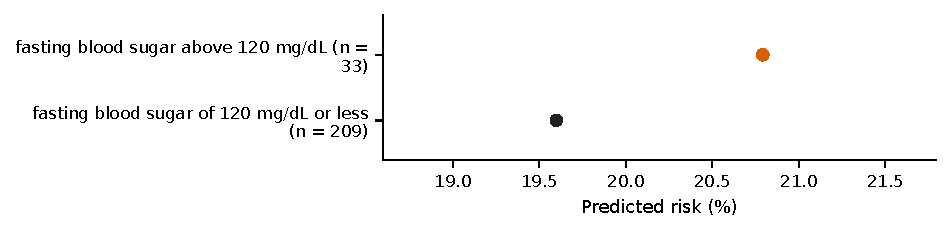
\includegraphics[width=\linewidth,height=0.88\textheight,keepaspectratio]{figures/heart-s5-c2/ann_37-categories-small.pdf}
\caption{High fasting sugar term: The predicted value for the typical case at each level, through this part (n = training patients; grey: fewer than 20).}
\label{fig:hearts5c2:plot-ann37-0}
\end{figure}
\begin{figure}[H]\centering
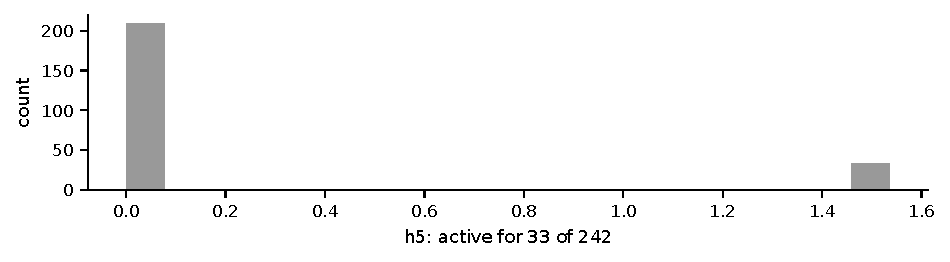
\includegraphics[width=\linewidth,height=0.88\textheight,keepaspectratio]{figures/heart-s5-c2/ann_37-units.pdf}
\caption{High fasting sugar term: This part's hidden units: each unit's output against its main numeric input (top) and how often it is active (bottom).}
\label{fig:hearts5c2:plot-ann37-1}
\end{figure}
\par\smallskip\noindent{\small Technical detail: \ref{tech:ann37}.\par}
\subsection{Not supported by the model}
\begin{itemize}\setlength\itemsep{0pt}\small
\item C16: direction claim about thallium stress test result in the whole model: not supported by the model (15\% of patients have the opposite sign (allowed: 10\%)).
\item C25: direction claim about resting ECG in the whole model: not supported by the model (34\% of patients have the opposite sign (allowed: 10\%)).
\item C28: direction claim about resting ECG in the whole model: not supported by the model (41\% of patients have the opposite sign (allowed: 10\%)).
\item C48: interaction claim about resting blood pressure and chest pain type in part ann\_\allowbreak{}34: not supported by the model (the group difference is below 0.1 log-odds).
\item C49: interaction claim about chest pain type and exercise-induced angina in part ann\_\allowbreak{}34: not supported by the model (the group difference is below 0.1 log-odds; the part's own counterfactual difference has the opposite sign).
\item C50: interaction claim about resting blood pressure and exercise-induced angina in part ann\_\allowbreak{}34: not supported by the model (the group difference is below 0.1 log-odds; the part's own counterfactual difference has the opposite sign).
\item C51: interaction claim about resting blood pressure and thallium stress test result in part ann\_\allowbreak{}34: not supported by the model (the group difference is below 0.1 log-odds; the part's own counterfactual difference has the opposite sign).
\item C62: null claim about resting ECG and exercise-induced angina in part ann\_\allowbreak{}36: not supported by the model (predictions move by up to 0.059).
\end{itemize}
\clearpage\section*{Technical detail: heart-s5-c2}
\addcontentsline{toc}{section}{Technical detail: heart-s5-c2}
\noindent{\small The record behind each part: the original hypothesis, the closed form, and every claim with its estimate (log-odds and odds ratio), range across patients, n and test check.\par}
\renewcommand{\thesubsection}{T.\arabic{subsection}}\setcounter{subsection}{0}
\subsection{The whole model}\label{tech:ann38}
\noindent{\footnotesize Annotation ann\_\allowbreak{}38 (heart\_\allowbreak{}disease\_\allowbreak{}logit). Reads: age, sex, chest pain type, resting blood pressure, serum cholesterol, fasting blood sugar, resting ECG, maximum heart rate reached during the exercise test, exercise-induced angina, ST depression during exercise (compared with rest), slope of the ST segment at peak exercise, number of major vessels coloured by fluoroscopy, thallium stress test result.\par}
\paragraph{Original hypothesis (unchanged).} Root: p = sigmoid(z), z = -0.487 + LINEAR CORE + 0.136*ischaemia\_\allowbreak{}gate + 0.252*bp\_\allowbreak{}offset\_\allowbreak{}gate - 0.118*\allowbreak{}ischaemia\_\allowbreak{}damping\_\allowbreak{}thal6 + 0.729*\allowbreak{}lvh\_\allowbreak{}without\_\allowbreak{}exercise\_\allowbreak{}angina + 0.048*\allowbreak{}high\_\allowbreak{}fasting\_\allowbreak{}sugar. LINEAR CORE (17 direct input-$>$output edges, z-scored inputs): ca +1.473, sex:0 -1.062, slope:1 -0.921, chol +0.522, trestbps +0.498, cp:1 -0.489, exang:1 +0.471, cp:3 -0.444, thal:3 -0.423, thal:6 -0.413, slope:3 -0.370, cp:4 +0.357, fbs:0 +0.264, thalach -0.226, restecg:0 -0.159, exang:0 +0.136, age +0.126. Five inputs are unconnected (sex:1, cp:2, restecg:1, slope:2, thal:7; zero-effect entries of this root). Oldpeak, thal:4, restecg:2 and fbs:1 have no direct edge and act only through the children. COMPOSITION: additive readouts, with a serial fan-out inside. ischaemia\_\allowbreak{}gate (oldpeak above a resting-ECG-dependent threshold) is read out directly and also feeds bp\_\allowbreak{}offset\_\allowbreak{}gate (the ischaemia score minus a resting-BP offset, the largest nonlinear readout) and ischaemia\_\allowbreak{}damping\_\allowbreak{}thal6 (a near-linear term that takes back part of the ischaemia score and adds a fixed-defect term); identity nodes identity\_\allowbreak{}290 and identity\_\allowbreak{}1416 carry those two links so each gate is its own leaf. Two independent indicators add to z: lvh\_\allowbreak{}without\_\allowbreak{}exercise\_\allowbreak{}angina (+0.236 for LVH on the resting ECG without exercise angina) and high\_\allowbreak{}fasting\_\allowbreak{}sugar (+0.074, negligible). EVIDENCE (train, n=242): full model AUC 0.9389, acc 0.880 (compute\_\allowbreak{}performance)\allowbreak{}. Linear core alone AUC 0.933; logit SD 3.19 (core) vs 0.57 (all hidden readouts). Removing the ischaemia gate with its downstream effects gives 0.932; readout-only ablations: ischaemia 0.938, BP 0.933, damping 0.938, LVH 0.939, fbs 0.939. Treating all five ReLUs as identities gives 0.917 (the gating matters); one least-squares linear fit of all hidden readouts on their inputs gives 0.938 (R2 0.84); an L2 logistic regression on all 26 inputs gives 0.936. Mean $|$SHAP$|$ (train, all 242): ca 0.145, sex:0 0.109, slope:1 0.108, thal:3 0.050, oldpeak 0.047, cp:3 0.045, exang:1 0.044, chol 0.043. Interpretation: close to logistic regression plus one ischaemia correction: ST depression raises risk only above a threshold that is lower with a normal resting ECG, more steeply when resting BP is low; LVH without exercise angina adds a little. Counter-directional signs reported, not explained: restecg:0 positive in the ischaemia gate, trestbps negative in the BP gate, thal:6 (fixed defect) negative directly, fbs:0 +0.26 directly. Same core design as the 10-seed heart-s5 record (key 9330) and the sibling cluster lead heart-s5-c1 (ischaemia gate -$>$ resting-BP gate), with a damping node, an LVH indicator and a fasting-sugar indicator instead of c1's age gate.
\paragraph{Closed form.} Read through its parts (their formulas are in their own sections).
\paragraph{Split inputs.} To annotate the parts, the explanation split these inputs into copies (a refactoring step that does not change what the model computes); the diagrams draw each input once: non-anginal pain (2 copies); exercise pain (3 copies); normal ECG (2 copies); fixed defect (3 copies); blood pressure (2 copies).
\paragraph{Evidence table} (next page, landscape).
\begin{landscape}
{\scriptsize\setlength{\tabcolsep}{3pt}\renewcommand{\arraystretch}{1.15}
\rowcolors{2}{black!6}{white}
\begin{longtable}{@{}l>{\raggedright\arraybackslash}p{0.36\linewidth}>{\raggedright\arraybackslash}p{0.14\linewidth}rrr>{\raggedright\arraybackslash}p{0.06\linewidth}>{\raggedright\arraybackslash}p{0.17\linewidth}c@{}}
\toprule\rowcolor{white}
ID & What is checked & Risk, typical patient & Log-odds & OR & Range (p10--p90) & n & Test check & OK \\
\midrule\endfirsthead
\toprule\rowcolor{white}
ID & What is checked & Risk, typical patient & Log-odds & OR & Range (p10--p90) & n & Test check & OK \\
\midrule\endhead
\bottomrule\endfoot
C01 & direction: number of vessels coloured by fluoroscopy: 0 vessels to 2 vessels (whole model) \newline{\itshape shape: steady (equal steps); 100\% of patients same; verified; risk saturates near 100\%} & 20\% to 87\% & 3.30 & 27.2 & 3.30 to 3.30 & 242 & unclear; AUC gain 0.025 [-0.049, 0.102] & \textcolor{OliveGreen}{yes} \\
C02 & direction: slope of the ST segment at peak exercise: an upsloping ST segment to a flat ST segment (whole model) \newline{\itshape shape: categorical; highest to lowest: a flat ST segment, a downsloping ST segment, an upsloping ST segment} & 20\% to 61\% & 1.84 & 6.32 & 1.84 to 1.84 & 115, 110 & disagrees; AUC gain -0.017 [-0.061, 0.016] & \textcolor{OliveGreen}{yes} \\
C03 & direction: ST depression on exercise: 0.0 mm to 2.8 mm (whole model) \newline{\itshape shape: hinge at 0.4 mm; 70\% of patients same; fallback} & 16\% to 50\% & 1.22 & 3.40 & 0.77 to 1.69 & 242 & unclear; AUC gain 0.009 [-0.008, 0.033] & \textcolor{OliveGreen}{yes} \\
C04 & direction: serum cholesterol: 193 mg/dL (5.0 mmol/L) to 308 mg/dL (8.0 mmol/L) (whole model) \newline{\itshape shape: steady; 100\% of patients same; verified} & 13\% to 34\% & 1.25 & 3.48 & 1.25 to 1.25 & 242 & disagrees; AUC gain -0.028 [-0.071, 0.002] & \textcolor{OliveGreen}{yes} \\
C05 & direction: resting blood pressure: 110 mm Hg to 155 mm Hg (direct contribution only, not through any part) \newline{\itshape shape: steady; 100\% of patients same; verified} & 12\% to 33\% & 1.23 & 3.43 & 1.23 to 1.23 & 242 & unclear; AUC gain 0.006 [-0.024, 0.037] & \textcolor{OliveGreen}{yes} \\
C06 & direction: chest pain type: no chest pain (asymptomatic) to typical angina (direct contribution only, not through any part) \newline{\itshape shape: categorical; highest to lowest: no chest pain (asymptomatic), atypical angina, non-anginal chest pain, typical angina} & 20\% to 2\% & -2.42 & 0.09 & -2.42 to -2.42 & 108, 22 & agrees; AUC gain 0.032 [0.008, 0.062] & \textcolor{OliveGreen}{yes} \\
C07 & direction: chest pain type: no chest pain (asymptomatic) to typical angina (whole model) \newline{\itshape shape: categorical; highest to lowest: no chest pain (asymptomatic), atypical angina, non-anginal chest pain, typical angina} & 20\% to 2\% & -2.42 & 0.09 & -2.42 to -2.42 & 108, 22 & agrees; AUC gain 0.032 [0.008, 0.062] & \textcolor{OliveGreen}{yes} \\
C08 & direction: sex: male to female (whole model) \newline{\itshape shape: categorical; highest to lowest: male, female} & 20\% to 3\% & -2.24 & 0.11 & -2.24 to -2.24 & 159, 83 & unclear; AUC gain 0.022 [-0.011, 0.065] & \textcolor{OliveGreen}{yes} \\
C09 & direction: thallium stress test result: a normal thallium scan to thallium stress test result other than a normal thallium scan, a fixed defect on the thallium scan (direct contribution only, not through any part) \newline{\itshape shape: categorical; highest to lowest: thallium stress test result other than a normal thallium scan, a fixed defect on the thallium scan, a normal thallium scan, a fixed defect on the thallium scan} & 20\% to 36\% & 0.85 & 2.34 & 0.85 to 0.85 & 135, 92 & unclear; AUC gain 0.013 [-0.011, 0.041] & \textcolor{OliveGreen}{yes} \\
C10 & direction: thallium stress test result: a normal thallium scan to a reversible defect on the thallium scan (whole model) \newline{\itshape shape: categorical; highest to lowest: a reversible defect on the thallium scan, thallium stress test result coded 4 (meaning not recorded), a normal thallium scan, a fixed defect on the thallium scan} & 20\% to 36\% & 0.85 & 2.34 & 0.85 to 0.85 & 135, 90 & unclear; AUC gain 0.014 [-0.009, 0.042] & \textcolor{OliveGreen}{yes} \\
C11 & direction: chest pain type: no chest pain (asymptomatic) to non-anginal chest pain (whole model) \newline{\itshape shape: categorical; highest to lowest: no chest pain (asymptomatic), atypical angina, non-anginal chest pain, typical angina} & 20\% to 4\% & -1.72 & 0.18 & -1.74 to -1.70 & 108, 70 & agrees; AUC gain 0.032 [0.008, 0.062] & \textcolor{OliveGreen}{yes} \\
C12 & direction: chest pain type: no chest pain (asymptomatic) to non-anginal chest pain (direct contribution only, not through any part) \newline{\itshape shape: categorical; highest to lowest: no chest pain (asymptomatic), atypical angina, non-anginal chest pain, typical angina} & 20\% to 4\% & -1.70 & 0.18 & -1.70 to -1.70 & 108, 70 & agrees; AUC gain 0.032 [0.008, 0.062] & \textcolor{OliveGreen}{yes} \\
C13 & direction: resting blood pressure: 110 mm Hg to 155 mm Hg (whole model) \newline{\itshape shape: accelerating; 75\% of patients same; fallback} & 15\% to 28\% & 0.97 & 2.63 & 0.75 to 1.15 & 242 & unclear; AUC gain 0.005 [-0.017, 0.031] & \textcolor{OliveGreen}{yes} \\
C14 & direction: exercise-induced angina: no chest pain on exercise to chest pain brought on by exercise (direct contribution only, not through any part) \newline{\itshape shape: categorical; highest to lowest: chest pain brought on by exercise, no chest pain on exercise} & 20\% to 33\% & 0.71 & 2.03 & 0.71 to 0.71 & 160, 82 & agrees; AUC gain 0.012 [0.001, 0.030] & \textcolor{OliveGreen}{yes} \\
C15 & direction: exercise-induced angina: no chest pain on exercise to chest pain brought on by exercise (whole model) \newline{\itshape shape: categorical; highest to lowest: chest pain brought on by exercise, no chest pain on exercise} & 20\% to 31\% & 0.55 & 1.73 & 0.39 to 0.71 & 160, 82 & unclear; AUC gain 0.008 [0.000, 0.022] & \textcolor{OliveGreen}{yes} \\
C16 & direction: thallium stress test result: a normal thallium scan to thallium stress test result coded 4 (meaning not recorded) (whole model) \newline{\itshape shape: categorical; highest to lowest: a reversible defect on the thallium scan, thallium stress test result coded 4 (meaning not recorded), a normal thallium scan, a fixed defect on the thallium scan} & 20\% to 31\% & 0.52 & 1.69 & -0.22 to 0.85 & 135, 2 (small n) & unclear; AUC gain 0.014 [-0.009, 0.042] & \textcolor{BrickRed}{no} \\
C17 & direction: thallium stress test result: a normal thallium scan to a fixed defect on the thallium scan (direct contribution only, not through any part) \newline{\itshape shape: categorical; highest to lowest: thallium stress test result other than a normal thallium scan, a fixed defect on the thallium scan, a normal thallium scan, a fixed defect on the thallium scan} & 20\% to 9\% & -0.86 & 0.42 & -0.86 to -0.86 & 135, 15 (small n) & unclear; AUC gain 0.013 [-0.011, 0.041] & \textcolor{OliveGreen}{yes} \\
C18 & direction: fasting blood sugar: fasting blood sugar of 120 mg/dL or less to fasting blood sugar above 120 mg/dL (direct contribution only, not through any part) \newline{\itshape shape: categorical; highest to lowest: fasting blood sugar of 120 mg/dL or less, fasting blood sugar above 120 mg/dL} & 20\% to 10\% & -0.77 & 0.46 & -0.77 to -0.77 & 209, 33 & disagrees; AUC gain -0.004 [-0.020, 0.009] & \textcolor{OliveGreen}{yes} \\
C19 & direction: maximum heart rate: 118 beats per minute to 175 beats per minute (whole model) \newline{\itshape shape: steady; 100\% of patients same; verified} & 26\% to 16\% & -0.57 & 0.56 & -0.57 to -0.57 & 242 & unclear; AUC gain 0.006 [0.000, 0.022] & \textcolor{OliveGreen}{yes} \\
C20 & direction: chest pain type: no chest pain (asymptomatic) to atypical angina (direct contribution only, not through any part) \newline{\itshape shape: categorical; highest to lowest: no chest pain (asymptomatic), atypical angina, non-anginal chest pain, typical angina} & 20\% to 11\% & -0.72 & 0.49 & -0.72 to -0.72 & 108, 42 & agrees; AUC gain 0.032 [0.008, 0.062] & \textcolor{OliveGreen}{yes} \\
C21 & direction: chest pain type: no chest pain (asymptomatic) to atypical angina (whole model) \newline{\itshape shape: categorical; highest to lowest: no chest pain (asymptomatic), atypical angina, non-anginal chest pain, typical angina} & 20\% to 11\% & -0.72 & 0.49 & -0.72 to -0.72 & 108, 42 & agrees; AUC gain 0.032 [0.008, 0.062] & \textcolor{OliveGreen}{yes} \\
C22 & direction: fasting blood sugar: fasting blood sugar of 120 mg/dL or less to fasting blood sugar above 120 mg/dL (whole model) \newline{\itshape shape: categorical; highest to lowest: fasting blood sugar of 120 mg/dL or less, fasting blood sugar above 120 mg/dL} & 20\% to 11\% & -0.69 & 0.50 & -0.69 to -0.69 & 209, 33 & disagrees; AUC gain -0.003 [-0.019, 0.009] & \textcolor{OliveGreen}{yes} \\
C23 & direction: thallium stress test result: a normal thallium scan to a fixed defect on the thallium scan (whole model) \newline{\itshape shape: categorical; highest to lowest: a reversible defect on the thallium scan, thallium stress test result coded 4 (meaning not recorded), a normal thallium scan, a fixed defect on the thallium scan} & 20\% to 11\% & -0.69 & 0.50 & -0.75 to -0.58 & 135, 15 (small n) & unclear; AUC gain 0.014 [-0.009, 0.042] & \textcolor{OliveGreen}{yes} \\
C24 & direction: slope of the ST segment at peak exercise: an upsloping ST segment to a downsloping ST segment (whole model) \newline{\itshape shape: categorical; highest to lowest: a flat ST segment, a downsloping ST segment, an upsloping ST segment} & 20\% to 27\% & 0.40 & 1.48 & 0.40 to 0.40 & 115, 17 (small n) & disagrees; AUC gain -0.017 [-0.061, 0.016] & \textcolor{OliveGreen}{yes} \\
C25 & direction: resting ECG: a normal resting ECG to signs of left ventricular hypertrophy on the resting ECG (whole model) \newline{\itshape shape: categorical; highest to lowest: signs of left ventricular hypertrophy on the resting ECG, an ST-T wave abnormality on the resting ECG, a normal resting ECG} & 20\% to 25\% & 0.21 & 1.24 & -0.32 to 0.55 & 121, 119 & disagrees; AUC gain -0.003 [-0.023, 0.013] & \textcolor{BrickRed}{no} \\
C26 & direction: resting ECG: a normal resting ECG to resting ECG other than a normal resting ECG (direct contribution only, not through any part) \newline{\itshape shape: categorical; highest to lowest: resting ECG other than a normal resting ECG, a normal resting ECG} & 20\% to 25\% & 0.32 & 1.37 & 0.32 to 0.32 & 121, 121 & unclear; AUC gain 0.000 [-0.016, 0.015] & \textcolor{OliveGreen}{yes} \\
C27 & direction: age: 42 years to 66 years (whole model) \newline{\itshape shape: steady; 100\% of patients same; verified} & 17\% to 22\% & 0.33 & 1.39 & 0.33 to 0.33 & 242 & disagrees; AUC gain -0.005 [-0.023, 0.01] & \textcolor{OliveGreen}{yes} \\
C28 & direction: resting ECG: a normal resting ECG to an ST-T wave abnormality on the resting ECG (whole model) \newline{\itshape shape: categorical; highest to lowest: signs of left ventricular hypertrophy on the resting ECG, an ST-T wave abnormality on the resting ECG, a normal resting ECG} & 20\% to 21\% & 0.06 & 1.06 & -0.32 to 0.32 & 121, 2 (small n) & disagrees; AUC gain -0.003 [-0.023, 0.013] & \textcolor{BrickRed}{no} \\
C29 & magnitude: number of vessels coloured by fluoroscopy: 0 vessels to 2 vessels, typical patient \newline{\itshape shape: steady (equal steps); 100\% of patients same; verified; risk saturates near 100\%} & 20\% to 87\% & 3.30 & 27.2 &  & 242 & unclear; AUC gain 0.025 [-0.049, 0.102] & \textcolor{OliveGreen}{yes} \\
C30 & magnitude: slope of the ST segment at peak exercise: an upsloping ST segment to a flat ST segment, typical patient \newline{\itshape shape: categorical; highest to lowest: a flat ST segment, a downsloping ST segment, an upsloping ST segment} & 20\% to 61\% & 1.84 & 6.32 &  & 115, 110 & disagrees; AUC gain -0.017 [-0.061, 0.016] & \textcolor{OliveGreen}{yes} \\
C31 & magnitude: ST depression on exercise: 0.0 mm to 2.8 mm, typical patient \newline{\itshape shape: hinge at 0.4 mm; 70\% of patients same; fallback} & 16\% to 50\% & 1.64 & 5.15 &  & 242 & unclear; AUC gain 0.009 [-0.008, 0.033] & \textcolor{OliveGreen}{yes} \\
C32 & magnitude: serum cholesterol: 193 mg/dL (5.0 mmol/L) to 308 mg/dL (8.0 mmol/L), typical patient \newline{\itshape shape: steady; 100\% of patients same; verified} & 13\% to 34\% & 1.25 & 3.48 &  & 242 & disagrees; AUC gain -0.028 [-0.071, 0.002] & \textcolor{OliveGreen}{yes} \\
C33 & magnitude: chest pain type: no chest pain (asymptomatic) to typical angina, typical patient \newline{\itshape shape: categorical; highest to lowest: no chest pain (asymptomatic), atypical angina, non-anginal chest pain, typical angina} & 20\% to 2\% & -2.42 & 0.09 &  & 108, 22 & agrees; AUC gain 0.032 [0.008, 0.062] & \textcolor{OliveGreen}{yes} \\
C34 & structure: made of ischaemia\_\allowbreak{}gate, bp\_\allowbreak{}offset\_\allowbreak{}gate, ischaemia\_\allowbreak{}damping\_\allowbreak{}thal6,\allowbreak{} lvh\_\allowbreak{}without\_\allowbreak{}exercise\_\allowbreak{}angina,\allowbreak{} high\_\allowbreak{}fasting\_\allowbreak{}sugar and inputs age, sex, cp, trestbps, chol, fbs, restecg, thalach, exang, slope, ca, thal; added; ann\_\allowbreak{}33 feeds ann\_\allowbreak{}34; ann\_\allowbreak{}33 feeds ann\_\allowbreak{}35 &  &  &  &  & 242 & train only & \textcolor{OliveGreen}{yes} \\
\end{longtable}}
\end{landscape}
\subsection{ST depression signal}\label{tech:ann33}
\noindent{\footnotesize Annotation ann\_\allowbreak{}33 (ischaemia\_\allowbreak{}gate). Reads: resting ECG, ST depression during exercise (compared with rest), thallium stress test result.\par}
\paragraph{Original hypothesis (unchanged).} Ischaemia-evidence gate (raises risk). 204 = ReLU(0.385 + 2.536*oldpeak + 0.992*restecg:0 - 0.876*thal:4). Hypothesis: a one-sided ST-depression score that opens above an oldpeak threshold set by the resting ECG (z-oldpeak -0.57 with a normal ECG, +0.21 without) and then rises with oldpeak; it adds 0.136 per unit to the logit directly, a further 0.286 per unit through the BP gate while that gate is open, and -0.099 per unit through the damping node, so about 0.32 logit per unit in all. EVIDENCE (train, n=242): active for 45\% (51\% with a normal ECG, 40\% without); corr with oldpeak 0.92; disease rate 60\% when active vs 32\% when inactive. Mean $|$sensitivity$|$ oldpeak 1.14 $>$ restecg:0 0.45 $>$ thal:4 0.39 (thal:4 has 2 patients). This is the main nonlinear effect: removing it with its downstream effects lowers train AUC 0.939 -$>$ 0.932 (below the linear-core level 0.933); an affine replacement recovers 0.938. Supported. Oldpeak and thal:4 have no direct edge and act only here. The positive restecg:0 weight (a normal ECG raises the score; restecg:0's direct edge is -0.16) is counter-intuitive and is reported, not explained.
\paragraph{Closed form} {\footnotesize(weights and biases at 3 significant figures; largest difference from the part on the training patients 1.77636e-15).}
{\small\begingroup\allowdisplaybreaks
\begin{align*}
y_{0} &= \operatorname{relu}\bigl(0.385 + 0.992 x_{restecg:0\_b} + 2.54 x_{oldpeak} \\
&\qquad - 0.876 x_{thal:4}\bigr)
\end{align*}\endgroup}

\paragraph{Evidence table} (next page, landscape).
\begin{landscape}
{\scriptsize\setlength{\tabcolsep}{3pt}\renewcommand{\arraystretch}{1.15}
\rowcolors{2}{black!6}{white}
\begin{longtable}{@{}l>{\raggedright\arraybackslash}p{0.36\linewidth}>{\raggedright\arraybackslash}p{0.14\linewidth}rrr>{\raggedright\arraybackslash}p{0.06\linewidth}>{\raggedright\arraybackslash}p{0.17\linewidth}c@{}}
\toprule\rowcolor{white}
ID & What is checked & Risk, typical patient & Log-odds & OR & Range (p10--p90) & n & Test check & OK \\
\midrule\endfirsthead
\toprule\rowcolor{white}
ID & What is checked & Risk, typical patient & Log-odds & OR & Range (p10--p90) & n & Test check & OK \\
\midrule\endhead
\bottomrule\endfoot
C35 & direction: ST depression on exercise: 0.0 mm to 2.8 mm (through this part) \newline{\itshape shape: hinge at 1.3 mm; 70\% of patients same; fallback; one point with C41 (median fold 1.3 mm, typical patient 0.4 mm, 10th-90th percentile 0.4 mm to 1.3 mm, wide)} & 16\% to 50\% & 1.22 & 3.40 & 0.77 to 1.69 & 242 & unclear; AUC gain 0.009 [-0.008, 0.033] & \textcolor{OliveGreen}{yes} \\
C36 & direction: resting ECG: a normal resting ECG to resting ECG other than a normal resting ECG (through this part) \newline{\itshape shape: categorical; highest to lowest: a normal resting ECG, resting ECG other than a normal resting ECG} & 20\% to 16\% & -0.26 & 0.77 & -0.64 to 0.00 & 121, 121 & disagrees; AUC gain -0.002 [-0.016, 0.012] & \textcolor{OliveGreen}{yes} \\
C37 & direction: thallium stress test result: thallium stress test result other than thallium stress test result coded 4 (meaning not recorded) to thallium stress test result coded 4 (meaning not recorded) (through this part) \newline{\itshape shape: categorical; highest to lowest: thallium stress test result other than thallium stress test result coded 4 (meaning not recorded), thallium stress test result coded 4 (meaning not recorded)} & 20\% to 16\% & -0.33 & 0.72 & -1.07 to 0.00 & 240, 2 (small n) & disagrees; AUC gain -0.001 [-0.006, 0.000] & \textcolor{OliveGreen}{yes} \\
C38 & interaction: effect of ST depression on exercise (0.0 mm to 2.8 mm) by thallium stress test result: thallium stress test result coded 4 (meaning not recorded) minus thallium stress test result other than thallium stress test result coded 4 (meaning not recorded); stronger in thallium stress test result other than thallium stress test result coded 4 (meaning not recorded) \newline{\itshape shape: hinge at 0.4 mm; 74\% of patients same; fallback} & thallium stress test result coded 4 (meaning not recorded): 31\% to 31\%; thallium stress test result other than thallium stress test result coded 4 (meaning not recorded): 16\% to 50\% & -1.23 & 0.29 &  & 2, 240 (small n) & unclear; AUC gain -0.001 [-0.006, 0.000] & \textcolor{OliveGreen}{yes} \\
C39 & interaction: effect of ST depression on exercise (0.0 mm to 2.8 mm) by resting ECG: resting ECG other than a normal resting ECG minus a normal resting ECG; stronger in a normal resting ECG \newline{\itshape shape: hinge at 0.4 mm; 57\% of patients same; fallback} & resting ECG other than a normal resting ECG: 25\% to 48\%; a normal resting ECG: 16\% to 50\% & -0.68 & 0.50 &  & 121, 121 & agrees; AUC gain -0.002 [-0.016, 0.012] & \textcolor{OliveGreen}{yes} \\
C40 & interaction: effect of thallium stress test result (thallium stress test result other than thallium stress test result coded 4 (meaning not recorded) to thallium stress test result coded 4 (meaning not recorded)) by resting ECG: resting ECG other than a normal resting ECG minus a normal resting ECG; stronger in resting ECG other than a normal resting ECG \newline{\itshape shape: categorical; highest to lowest: thallium stress test result other than thallium stress test result coded 4 (meaning not recorded), thallium stress test result coded 4 (meaning not recorded)} & resting ECG other than a normal resting ECG: 25\% to 44\%; a normal resting ECG: 20\% to 31\% & 0.14 & 1.16 &  & 121, 121, 2 (small n) & unclear; AUC gain -0.002 [-0.016, 0.012] & \textcolor{OliveGreen}{yes} \\
C41 & threshold: ST depression on exercise: fold at about 1.3 mm (starts) \newline{\itshape shape: hinge at 1.3 mm; 70\% of patients same; fallback; one point with C41 (median fold 1.3 mm, typical patient 0.4 mm, 10th-90th percentile 0.4 mm to 1.3 mm, wide)} & 16\% to 62\% (typical patient with a fold) & 1.70 & 5.47 & 1.25 to 2.17 & 242, 109 & unclear; AUC gain 0.009 [-0.008, 0.033] & \textcolor{OliveGreen}{yes} \\
C42 & subgroup: who this part acts on: 109 of 242 patients & 76\% to 89\% (typical patient this part acts on (risk without the part, then with it)) & 0.74 & 2.09 & 0.02 to 1.62 & 109, 133 & unclear; AUC gain 0.006 [-0.014, 0.032] & \textcolor{OliveGreen}{yes} \\
C43 & structure: its formula reproduces it on 242 training patients (largest difference 1.77636e-15) &  & 2e-15 &  &  & 242 & train only & \textcolor{OliveGreen}{yes} \\
\end{longtable}}
\end{landscape}
\subsection{Blood pressure step}\label{tech:ann34}
\noindent{\footnotesize Annotation ann\_\allowbreak{}34 (bp\_\allowbreak{}offset\_\allowbreak{}gate). Reads: chest pain type, resting blood pressure, exercise-induced angina, thallium stress test result.\par}
\paragraph{Original hypothesis (unchanged).} Blood-pressure offset gate on the ischaemia score (raises risk). 290 = ReLU(-0.447 + 1.137*ischaemia\_\allowbreak{}gate - 0.773*trestbps - 0.153*exang:1 - 0.069*cp:3 - 0.007*thal:6), read out +0.252. Hypothesis: passes the ischaemia score on, minus an offset that grows with resting blood pressure (and slightly with exercise angina and non-anginal pain). With the ischaemia gate closed it still opens for low resting blood pressure, so within this gate lower resting BP raises risk (0.252*0.773 = 0.195 per SD while open), partly offsetting trestbps's direct +0.50 edge. EVIDENCE (train, n=242): active for 60\% (87\% with the ischaemia gate open, 38\% without); with the ischaemia gate open, active for 100\%, 85\% and 77\% of the low, middle and high resting-BP groups. Disease rate 50\% when active vs 35\% when inactive. Mean $|$sensitivity$|$ ischaemia score 0.60 $>$ trestbps 0.46 $>$ exang:1 0.09 $>$ cp:3 0.04 $>$ thal:6 0.004. It is the largest nonlinear readout (logit SD 0.50): readout ablation lowers train AUC 0.939 -$>$ 0.933; an affine replacement fits it well (R2 0.97, AUC 0.939), so its nonlinearity matters little. Supported. The negative BP term inside a risk-raising gate is reported, not explained.
\paragraph{Closed form} {\footnotesize(weights and biases at 3 significant figures; largest difference from the part on the training patients 1.77636e-15).}
{\small\begingroup\allowdisplaybreaks
\begin{align*}
y_{0} &= \operatorname{relu}\bigl(-0.447 + 1.0 x_{identity\_290} - 0.0688 x_{cp:3\_b} \\
&\qquad - 0.153 x_{exang:1\_b} - 0.00683 x_{thal:6\_b} - 0.773 x_{trestbps\_b}\bigr)
\end{align*}\endgroup}

\paragraph{Evidence table} (next page, landscape).
\begin{landscape}
{\scriptsize\setlength{\tabcolsep}{3pt}\renewcommand{\arraystretch}{1.15}
\rowcolors{2}{black!6}{white}
\begin{longtable}{@{}l>{\raggedright\arraybackslash}p{0.36\linewidth}>{\raggedright\arraybackslash}p{0.14\linewidth}rrr>{\raggedright\arraybackslash}p{0.06\linewidth}>{\raggedright\arraybackslash}p{0.17\linewidth}c@{}}
\toprule\rowcolor{white}
ID & What is checked & Risk, typical patient & Log-odds & OR & Range (p10--p90) & n & Test check & OK \\
\midrule\endfirsthead
\toprule\rowcolor{white}
ID & What is checked & Risk, typical patient & Log-odds & OR & Range (p10--p90) & n & Test check & OK \\
\midrule\endhead
\bottomrule\endfoot
C44 & direction: resting blood pressure: 110 mm Hg to 155 mm Hg (through this part) \newline{\itshape shape: hinge at 125 mm Hg; 75\% of patients same; fallback; one point with C52 (median fold 125 mm Hg, typical patient 148 mm Hg, 10th-90th percentile 122 mm Hg to 165 mm Hg, wide)} & 23\% to 17\% & -0.27 & 0.77 & -0.48 to -0.08 & 242 & disagrees; AUC gain -0.003 [-0.014, 0.004] & \textcolor{OliveGreen}{yes} \\
C45 & direction: exercise-induced angina: no chest pain on exercise to chest pain brought on by exercise (through this part) \newline{\itshape shape: categorical; highest to lowest: no chest pain on exercise, chest pain brought on by exercise} & 20\% to 18\% & -0.04 & 0.96 & -0.08 to 0.00 & 160, 82 & disagrees; AUC gain -0.001 [-0.006, 0.000] & \textcolor{OliveGreen}{yes} \\
C46 & direction: chest pain type: chest pain type other than non-anginal chest pain to non-anginal chest pain (through this part) \newline{\itshape shape: categorical; highest to lowest: chest pain type other than non-anginal chest pain, non-anginal chest pain} & 20\% to 19\% & -0.02 & 0.98 & -0.04 to 0.00 & 172, 70 & unclear; AUC gain 0.000 [0.000, 0.000] & \textcolor{OliveGreen}{yes} \\
C47 & direction: thallium stress test result: thallium stress test result other than a fixed defect on the thallium scan to a fixed defect on the thallium scan (through this part) \newline{\itshape shape: categorical; highest to lowest: thallium stress test result other than a fixed defect on the thallium scan, a fixed defect on the thallium scan} & 20\% to 19\% & -0.004 & 1.00 & -0.007 to 0.00 & 227, 15 (small n) & unclear; AUC gain 0.000 [0.000, 0.000] & \textcolor{OliveGreen}{yes} \\
C48 & interaction: effect of resting blood pressure (110 mm Hg to 155 mm Hg) by chest pain type: non-anginal chest pain minus chest pain type other than non-anginal chest pain; stronger in non-anginal chest pain \newline{\itshape shape: accelerating; 84\% of patients same; fallback; risk saturates near 0\%} & non-anginal chest pain: 3\% to 7\%; chest pain type other than non-anginal chest pain: 15\% to 28\% & 0.06 & 1.06 &  & 70, 172 & unclear; AUC gain 0.000 [0.000, 0.000] & \textcolor{BrickRed}{no} \\
C49 & interaction: effect of chest pain type (chest pain type other than non-anginal chest pain to non-anginal chest pain) by exercise-induced angina: chest pain brought on by exercise minus no chest pain on exercise; stronger in chest pain brought on by exercise \newline{\itshape shape: categorical; highest to lowest: chest pain type other than non-anginal chest pain, non-anginal chest pain} & chest pain brought on by exercise: 31\% to 7\%; no chest pain on exercise: 20\% to 4\% & -0.001 & 1.00 &  & 82, 160 & unclear; AUC gain -0.001 [-0.006, 0.000] & \textcolor{BrickRed}{no} \\
C50 & interaction: effect of resting blood pressure (110 mm Hg to 155 mm Hg) by exercise-induced angina: chest pain brought on by exercise minus no chest pain on exercise; stronger in no chest pain on exercise \newline{\itshape shape: accelerating; 81\% of patients same; fallback} & chest pain brought on by exercise: 25\% to 45\%; no chest pain on exercise: 15\% to 28\% & -0.05 & 0.95 &  & 82, 160 & unclear; AUC gain -0.001 [-0.006, 0.000] & \textcolor{BrickRed}{no} \\
C51 & interaction: effect of resting blood pressure (110 mm Hg to 155 mm Hg) by thallium stress test result: a fixed defect on the thallium scan minus thallium stress test result other than a fixed defect on the thallium scan; stronger in thallium stress test result other than a fixed defect on the thallium scan \newline{\itshape shape: accelerating; 76\% of patients same; fallback} & a fixed defect on the thallium scan: 8\% to 17\%; thallium stress test result other than a fixed defect on the thallium scan: 15\% to 28\% & -0.05 & 0.95 &  & 15, 227 (small n) & unclear; AUC gain 0.000 [0.000, 0.000] & \textcolor{BrickRed}{no} \\
C52 & threshold: resting blood pressure: fold at about 125 mm Hg (stops) for patients without chest pain on exercise \newline{\itshape shape: hinge at 125 mm Hg; 92\% of patients same; verified; risk saturates near 0\%; one point with C52 (median fold 125 mm Hg, typical patient 122 mm Hg, 10th-90th percentile 122 mm Hg to 165 mm Hg, wide)} & 4\% to 3\% (typical patient with a fold (patients without chest pain on exercise)) & -0.30 & 0.74 & -0.63 to -0.17 & 143, 78 & disagrees; AUC gain -0.003 [-0.014, 0.004] & \textcolor{OliveGreen}{yes} \\
C53 & subgroup: who this part acts on: 145 of 242 patients & 51\% to 68\% (typical patient this part acts on (risk without the part, then with it)) & 0.52 & 1.69 & 0.03 to 1.22 & 145, 97 & unclear; AUC gain 0.004 [-0.013, 0.024] & \textcolor{OliveGreen}{yes} \\
C54 & structure: its formula reproduces it on 242 training patients (largest difference 1.77636e-15) &  & 2e-15 &  &  & 242 & train only & \textcolor{OliveGreen}{yes} \\
\end{longtable}}
\end{landscape}
\subsection{Damping term}\label{tech:ann35}
\noindent{\footnotesize Annotation ann\_\allowbreak{}35 (ischaemia\_\allowbreak{}damping\_\allowbreak{}thal6). Reads: thallium stress test result.\par}
\paragraph{Original hypothesis (unchanged).} Ischaemia damping with a fixed-defect term (near-linear, small). 1416 = ReLU(0.853 + 0.841*ischaemia\_\allowbreak{}gate - 0.594*thal:6), read out -0.118. Hypothesis: almost always open, so it acts as a linear correction: it subtracts 0.099 per unit of the ischaemia score from the logit (damping the ischaemia gate's direct +0.136) and adds 0.070 per SD of thal:6 (about +0.29 logit for a fixed thallium defect, against thal:6's direct -0.41 edge). It closes only for fixed-defect patients whose ischaemia score is below 1.73. EVIDENCE (train, n=242): active for 97\% (closed for 8 of the 15 fixed-defect patients). Mean $|$sensitivity$|$ ischaemia score 0.97, thal:6 0.57. Readout ablation: train AUC 0.939 -$>$ 0.938; affine replacement R2 0.99, AUC 0.939. Supported; effectively linear.
\paragraph{Closed form} {\footnotesize(weights and biases at 3 significant figures; largest difference from the part on the training patients 2.22045e-16).}
{\small\begingroup\allowdisplaybreaks
\begin{align*}
y_{0} &= \operatorname{relu}\bigl(0.853 + 1.0 x_{identity\_1416} - 0.594 x_{thal:6\_c}\bigr)
\end{align*}\endgroup}

\paragraph{Evidence table} (next page, landscape).
\begin{landscape}
{\scriptsize\setlength{\tabcolsep}{3pt}\renewcommand{\arraystretch}{1.15}
\rowcolors{2}{black!6}{white}
\begin{longtable}{@{}l>{\raggedright\arraybackslash}p{0.36\linewidth}>{\raggedright\arraybackslash}p{0.14\linewidth}rrr>{\raggedright\arraybackslash}p{0.06\linewidth}>{\raggedright\arraybackslash}p{0.17\linewidth}c@{}}
\toprule\rowcolor{white}
ID & What is checked & Risk, typical patient & Log-odds & OR & Range (p10--p90) & n & Test check & OK \\
\midrule\endfirsthead
\toprule\rowcolor{white}
ID & What is checked & Risk, typical patient & Log-odds & OR & Range (p10--p90) & n & Test check & OK \\
\midrule\endhead
\bottomrule\endfoot
C55 & direction: thallium stress test result: thallium stress test result other than a fixed defect on the thallium scan to a fixed defect on the thallium scan (through this part) \newline{\itshape shape: categorical; highest to lowest: a fixed defect on the thallium scan, thallium stress test result other than a fixed defect on the thallium scan} & 20\% to 23\% & 0.18 & 1.20 & 0.12 to 0.29 & 227, 15 (small n) & unclear; AUC gain 0.002 [0.000, 0.01] & \textcolor{OliveGreen}{yes} \\
C56 & subgroup: who this part acts on: 234 of 242 patients & 24\% to 20\% (typical patient this part acts on (risk without the part, then with it)) & -0.23 & 0.79 & -0.48 to -0.12 & 234, 8 & unclear; AUC gain 0.000 [-0.011, 0.01] & \textcolor{OliveGreen}{yes} \\
C57 & structure: its formula reproduces it on 242 training patients (largest difference 2.22045e-16) &  & 2e-16 &  &  & 242 & train only & \textcolor{OliveGreen}{yes} \\
\end{longtable}}
\end{landscape}
\subsection{Hypertrophy without exercise pain}\label{tech:ann36}
\noindent{\footnotesize Annotation ann\_\allowbreak{}36 (lvh\_\allowbreak{}without\_\allowbreak{}exercise\_\allowbreak{}angina). Reads: resting ECG, exercise-induced angina.\par}
\paragraph{Original hypothesis (unchanged).} LVH without exercise angina (AND indicator, raises risk, small). 1611 = ReLU(-1.261 + 0.887*restecg:2 - 0.953*exang:1), read out +0.729. Hypothesis: a binary AND: open (constant 0.324, +0.236 logit) only for patients with left ventricular hypertrophy on the resting ECG and no exercise-induced angina, zero otherwise. EVIDENCE (train, n=242): active for exactly the 74 patients with LVH and no exercise angina; their disease rate is 41\%, against 20\% for patients with neither. Mean $|$sensitivity$|$ exang:1 0.29, restecg:2 0.27. Readout ablation: train AUC 0.939 -$>$ 0.939 (-0.0003). restecg:2 acts only here. Supported; near-negligible for ranking.
\paragraph{Closed form} {\footnotesize(weights and biases at 3 significant figures; largest difference from the part on the training patients 0.0).}
{\small\begingroup\allowdisplaybreaks
\begin{align*}
y_{0} &= \operatorname{relu}\bigl(-1.26 + 0.887 x_{restecg:2} - 0.953 x_{exang:1\_c}\bigr)
\end{align*}\endgroup}

\paragraph{Evidence table} (next page, landscape).
\begin{landscape}
{\scriptsize\setlength{\tabcolsep}{3pt}\renewcommand{\arraystretch}{1.15}
\rowcolors{2}{black!6}{white}
\begin{longtable}{@{}l>{\raggedright\arraybackslash}p{0.36\linewidth}>{\raggedright\arraybackslash}p{0.14\linewidth}rrr>{\raggedright\arraybackslash}p{0.06\linewidth}>{\raggedright\arraybackslash}p{0.17\linewidth}c@{}}
\toprule\rowcolor{white}
ID & What is checked & Risk, typical patient & Log-odds & OR & Range (p10--p90) & n & Test check & OK \\
\midrule\endfirsthead
\toprule\rowcolor{white}
ID & What is checked & Risk, typical patient & Log-odds & OR & Range (p10--p90) & n & Test check & OK \\
\midrule\endhead
\bottomrule\endfoot
C58 & direction: exercise-induced angina: no chest pain on exercise to chest pain brought on by exercise (through this part) \newline{\itshape shape: categorical; highest to lowest: no chest pain on exercise, chest pain brought on by exercise} & 30\% to 25\% (typical patient this part acts on) & -0.12 & 0.89 & -0.24 to 0.00 & 160, 82 & disagrees; AUC gain -0.003 [-0.013, 0.000] & \textcolor{OliveGreen}{yes} \\
C59 & direction: resting ECG: resting ECG other than signs of left ventricular hypertrophy on the resting ECG to signs of left ventricular hypertrophy on the resting ECG (through this part) \newline{\itshape shape: categorical; highest to lowest: signs of left ventricular hypertrophy on the resting ECG, resting ECG other than signs of left ventricular hypertrophy on the resting ECG} & 20\% to 24\% & 0.16 & 1.17 & 0.00 to 0.24 & 123, 119 & unclear; AUC gain 0.001 [-0.01, 0.012] & \textcolor{OliveGreen}{yes} \\
C60 & interaction: effect of exercise-induced angina (no chest pain on exercise to chest pain brought on by exercise) by resting ECG: signs of left ventricular hypertrophy on the resting ECG minus resting ECG other than signs of left ventricular hypertrophy on the resting ECG; stronger in resting ECG other than signs of left ventricular hypertrophy on the resting ECG \newline{\itshape shape: categorical; highest to lowest: chest pain brought on by exercise, no chest pain on exercise} & signs of left ventricular hypertrophy on the resting ECG: 25\% to 35\%; resting ECG other than signs of left ventricular hypertrophy on the resting ECG: 20\% to 31\% & -0.22 & 0.80 &  & 119, 123 & agrees; AUC gain 0.001 [-0.01, 0.012] & \textcolor{OliveGreen}{yes} \\
C61 & subgroup: who this part acts on: 74 of 242 patients & 25\% to 30\% (typical patient this part acts on (risk without the part, then with it)) & 0.24 & 1.27 & 0.24 to 0.24 & 74, 168 & disagrees; AUC gain -0.002 [-0.016, 0.006] & \textcolor{OliveGreen}{yes} \\
C62 & null: this part barely changes predictions (switched off) &  & 0.06 &  &  & 242 & train only & \textcolor{BrickRed}{no} \\
C63 & structure: its formula reproduces it on 242 training patients (largest difference 0.0) &  & 0.00 &  &  & 242 & train only & \textcolor{OliveGreen}{yes} \\
\end{longtable}}
\end{landscape}
\subsection{High fasting sugar term}\label{tech:ann37}
\noindent{\footnotesize Annotation ann\_\allowbreak{}37 (high\_\allowbreak{}fasting\_\allowbreak{}sugar). Reads: fasting blood sugar.\par}
\paragraph{Original hypothesis (unchanged).} High fasting blood sugar indicator (negligible). 3884 = ReLU(-0.980 + fbs:1), read out +0.048: +0.074 logit for the 33 patients with fasting blood sugar $>$ 120 mg/dl. Hypothesis: a small additive term for high fasting sugar (exactly linear on the two values of fbs:1); together with fbs:0's direct +0.26 edge, high fasting sugar overall lowers the logit (fbs:0 is the normal-sugar flag). EVIDENCE (train, n=242): active for exactly the 33 high-sugar patients; disease rate 45\% vs 44\%. Readout ablation changes train AUC by less than 0.0001; affine replacement R2 1.0. Supported; negligible.
\paragraph{Closed form} {\footnotesize(weights and biases at 3 significant figures; largest difference from the part on the training patients 0.0).}
{\small\begingroup\allowdisplaybreaks
\begin{align*}
y_{0} &= \operatorname{relu}\bigl(-0.98 + 1.0 x_{fbs:1}\bigr)
\end{align*}\endgroup}

\paragraph{Evidence table} (next page, landscape).
\begin{landscape}
{\scriptsize\setlength{\tabcolsep}{3pt}\renewcommand{\arraystretch}{1.15}
\rowcolors{2}{black!6}{white}
\begin{longtable}{@{}l>{\raggedright\arraybackslash}p{0.36\linewidth}>{\raggedright\arraybackslash}p{0.14\linewidth}rrr>{\raggedright\arraybackslash}p{0.06\linewidth}>{\raggedright\arraybackslash}p{0.17\linewidth}c@{}}
\toprule\rowcolor{white}
ID & What is checked & Risk, typical patient & Log-odds & OR & Range (p10--p90) & n & Test check & OK \\
\midrule\endfirsthead
\toprule\rowcolor{white}
ID & What is checked & Risk, typical patient & Log-odds & OR & Range (p10--p90) & n & Test check & OK \\
\midrule\endhead
\bottomrule\endfoot
C64 & direction: fasting blood sugar: fasting blood sugar of 120 mg/dL or less to fasting blood sugar above 120 mg/dL (through this part) \newline{\itshape shape: categorical; highest to lowest: fasting blood sugar above 120 mg/dL, fasting blood sugar of 120 mg/dL or less} & 20\% to 21\% & 0.07 & 1.08 & 0.07 to 0.07 & 209, 33 & unclear; AUC gain 0.000 [-0.005, 0.004] & \textcolor{OliveGreen}{yes} \\
C65 & subgroup: who this part acts on: 33 of 242 patients & 24\% to 25\% (typical patient this part acts on (risk without the part, then with it)) & 0.07 & 1.08 & 0.07 to 0.07 & 33, 209 & unclear; AUC gain 0.000 [-0.005, 0.004] & \textcolor{OliveGreen}{yes} \\
C66 & null: this part barely changes predictions (switched off) &  & 0.02 &  &  & 242 & train only & \textcolor{OliveGreen}{yes} \\
C67 & structure: its formula reproduces it on 242 training patients (largest difference 0.0) &  & 0.00 &  &  & 242 & train only & \textcolor{OliveGreen}{yes} \\
\end{longtable}}
\end{landscape}
\subsection*{The network before any explanation}\addcontentsline{toc}{subsection}{The network before any explanation} Figure~\ref{fig:hearts5c2:raw} (next page, landscape) is the trained network as it is, with no parts, no splits and no inserted units: inputs at the bottom, hidden units by depth, the output at the top, every connection drawn, every input column its own node (one-hot levels included).
\begin{landscape}
\begin{figure}[p]\centering
\resizebox{\linewidth}{!}{%
\definecolor{netup}{HTML}{D95F02}\definecolor{netdown}{HTML}{1B9E77}\definecolor{netmixed}{HTML}{7F7F7F}%
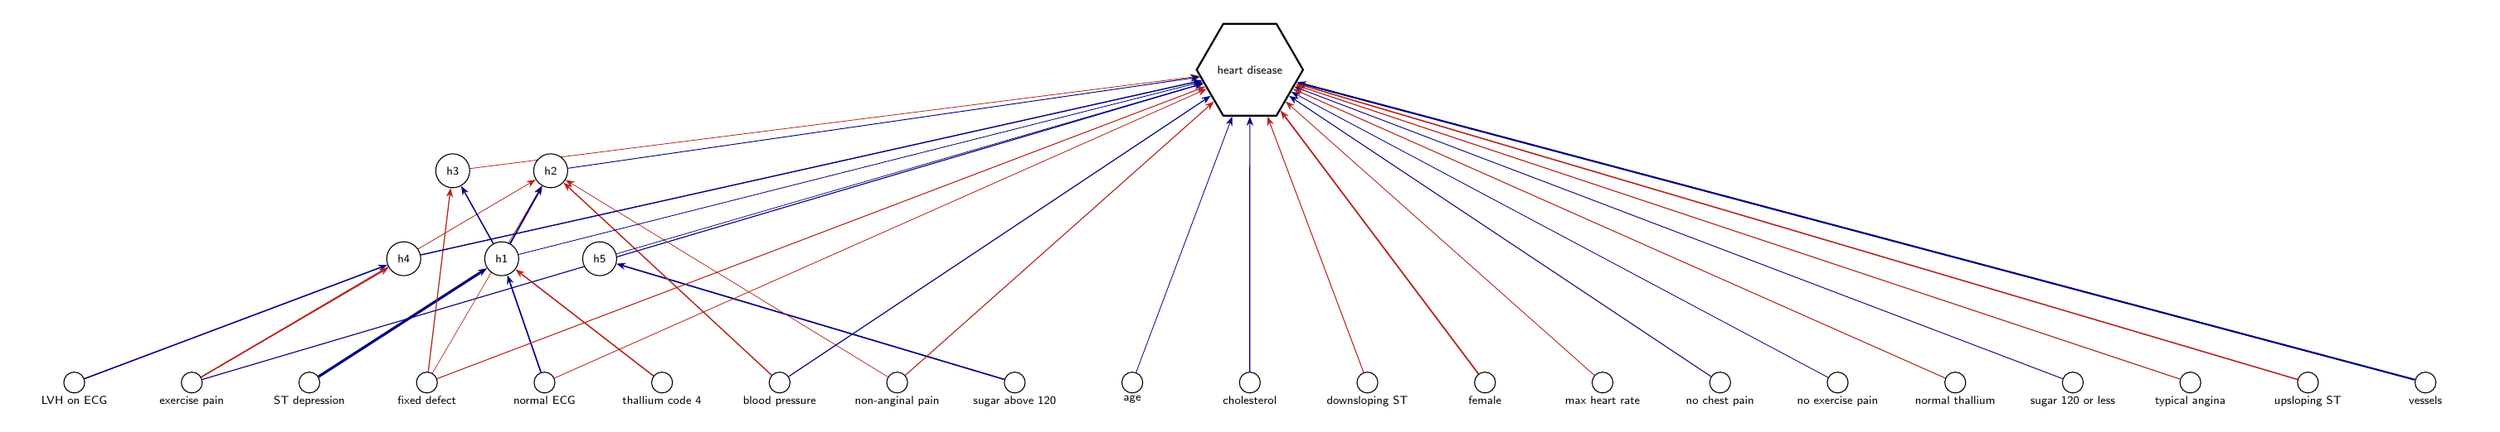
\begin{tikzpicture}[
  font=\sffamily\scriptsize, >={Stealth[length=1.4mm]},
  inp/.style={draw, circle, fill=white, minimum size=3.2mm, inner sep=0pt},
  hid/.style={draw, circle, fill=white, minimum size=5.2mm, inner sep=0.5pt, font=\sffamily\tiny},
  exitbox/.style={draw, thick, rectangle, fill=white, align=center, text width=17mm, minimum height=5mm, inner sep=1.5pt, font=\sffamily\tiny},
  sumbox/.style={draw, thick, dashed, rectangle, fill=white, align=center, text width=17mm, minimum height=5mm, inner sep=1.5pt, font=\sffamily\tiny},
  outp/.style={draw, thick, regular polygon, regular polygon sides=6, fill=white, minimum size=10mm, inner sep=0pt, font=\sffamily\tiny, align=center},
  stub/.style={draw, dashed, rounded corners=2pt, fill=white, align=center, inner sep=2pt, font=\sffamily\tiny, text width=15mm},
  inlab/.style={font=\sffamily\tiny, align=center, text width=15mm, inner sep=1pt, fill=white, fill opacity=0.8, text opacity=1},
  wpos/.style={draw=NavyBlue}, wneg/.style={draw=BrickRed}, wagg/.style={draw=black!45, line width=1.2pt},
  wmix/.style={draw=Plum},
]
\node[inp] (ninxxage) at (16.2,0.0) {};
\path (ninxxage.south) node[inlab, anchor=north] (labninxxage) {age};
\node[inp] (ninxxfbsx0) at (30.6,0.0) {};
\path (ninxxfbsx0.south) node[inlab, anchor=north] (labninxxfbsx0) {sugar 120 or less};
\node[inp] (ninxxfbsx1) at (14.4,0.0) {};
\path (ninxxfbsx1.south) node[inlab, anchor=north] (labninxxfbsx1) {sugar above 120};
\node[inp] (ninxxrestecgx0) at (7.2,0.0) {};
\path (ninxxrestecgx0.south) node[inlab, anchor=north] (labninxxrestecgx0) {normal ECG};
\node[inp] (ninxxrestecgx2) at (0.0,0.0) {};
\path (ninxxrestecgx2.south) node[inlab, anchor=north] (labninxxrestecgx2) {LVH on ECG};
\node[inp] (ninxxthalach) at (23.4,0.0) {};
\path (ninxxthalach.south) node[inlab, anchor=north] (labninxxthalach) {max heart rate};
\node[inp] (ninxxexangx0) at (27.0,0.0) {};
\path (ninxxexangx0.south) node[inlab, anchor=north] (labninxxexangx0) {no exercise pain};
\node[inp] (ninxxexangx1) at (1.8,0.0) {};
\path (ninxxexangx1.south) node[inlab, anchor=north] (labninxxexangx1) {exercise pain};
\node[inp] (ninxxoldpeak) at (3.6,0.0) {};
\path (ninxxoldpeak.south) node[inlab, anchor=north] (labninxxoldpeak) {ST depression};
\node[inp] (ninxxslopex1) at (34.2,0.0) {};
\path (ninxxslopex1.south) node[inlab, anchor=north] (labninxxslopex1) {upsloping ST};
\node[inp] (ninxxsexx0) at (21.6,0.0) {};
\path (ninxxsexx0.south) node[inlab, anchor=north] (labninxxsexx0) {female};
\node[inp] (ninxxslopex3) at (19.8,0.0) {};
\path (ninxxslopex3.south) node[inlab, anchor=north] (labninxxslopex3) {downsloping ST};
\node[inp] (ninxxca) at (36.0,0.0) {};
\path (ninxxca.south) node[inlab, anchor=north] (labninxxca) {vessels};
\node[inp] (ninxxthalx3) at (28.8,0.0) {};
\path (ninxxthalx3.south) node[inlab, anchor=north] (labninxxthalx3) {normal thallium};
\node[inp] (ninxxthalx4) at (9.0,0.0) {};
\path (ninxxthalx4.south) node[inlab, anchor=north] (labninxxthalx4) {thallium code 4};
\node[inp] (ninxxthalx6) at (5.4,0.0) {};
\path (ninxxthalx6.south) node[inlab, anchor=north] (labninxxthalx6) {fixed defect};
\node[inp] (ninxxcpx1) at (32.4,0.0) {};
\path (ninxxcpx1.south) node[inlab, anchor=north] (labninxxcpx1) {typical angina};
\node[inp] (ninxxcpx3) at (12.6,0.0) {};
\path (ninxxcpx3.south) node[inlab, anchor=north] (labninxxcpx3) {non-anginal pain};
\node[inp] (ninxxcpx4) at (25.2,0.0) {};
\path (ninxxcpx4.south) node[inlab, anchor=north] (labninxxcpx4) {no chest pain};
\node[inp] (ninxxtrestbps) at (10.8,0.0) {};
\path (ninxxtrestbps.south) node[inlab, anchor=north] (labninxxtrestbps) {blood pressure};
\node[inp] (ninxxchol) at (18.0,0.0) {};
\path (ninxxchol.south) node[inlab, anchor=north] (labninxxchol) {cholesterol};
\node[outp] (n0) at (18.0,4.8) {heart disease};
\node[hid] (n1416) at (5.795,3.25) {h3};
\node[hid] (n1611) at (5.045,1.9) {h4};
\node[hid] (n204) at (6.545,1.9) {h1};
\node[hid] (n290) at (7.295,3.25) {h2};
\node[hid] (n3884) at (8.045,1.9) {h5};
\begin{scope}[on background layer]
\draw[->, wpos, line width=0.29pt] (ninxxage) -- (n0);
\draw[->, wpos, line width=0.34pt] (ninxxfbsx0) -- (n0);
\draw[->, wpos, line width=0.60pt] (ninxxfbsx1) -- (n3884);
\draw[->, wneg, line width=0.31pt] (ninxxrestecgx0) -- (n0);
\draw[->, wpos, line width=0.60pt] (ninxxrestecgx0) -- (n204);
\draw[->, wpos, line width=0.56pt] (ninxxrestecgx2) -- (n1611);
\draw[->, wneg, line width=0.33pt] (ninxxthalach) -- (n0);
\draw[->, wpos, line width=0.30pt] (ninxxexangx0) -- (n0);
\draw[->, wpos, line width=0.41pt] (ninxxexangx1) -- (n0);
\draw[->, wneg, line width=0.58pt] (ninxxexangx1) -- (n1611);
\draw[->, wneg, line width=0.30pt] (ninxxexangx1) -- (n290);
\draw[->, wpos, line width=1.14pt] (ninxxoldpeak) -- (n204);
\draw[->, wneg, line width=0.57pt] (ninxxslopex1) -- (n0);
\draw[->, wneg, line width=0.62pt] (ninxxsexx0) -- (n0);
\draw[->, wneg, line width=0.38pt] (ninxxslopex3) -- (n0);
\draw[->, wpos, line width=0.77pt] (ninxxca) -- (n0);
\draw[->, wneg, line width=0.40pt] (ninxxthalx3) -- (n0);
\draw[->, wneg, line width=0.56pt] (ninxxthalx4) -- (n204);
\draw[->, wneg, line width=0.39pt] (ninxxthalx6) -- (n0);
\draw[->, wneg, line width=0.46pt] (ninxxthalx6) -- (n1416);
\draw[->, wneg, line width=0.25pt] (ninxxthalx6) -- (n290);
\draw[->, wneg, line width=0.42pt] (ninxxcpx1) -- (n0);
\draw[->, wneg, line width=0.41pt] (ninxxcpx3) -- (n0);
\draw[->, wneg, line width=0.27pt] (ninxxcpx3) -- (n290);
\draw[->, wpos, line width=0.38pt] (ninxxcpx4) -- (n0);
\draw[->, wpos, line width=0.42pt] (ninxxtrestbps) -- (n0);
\draw[->, wneg, line width=0.52pt] (ninxxtrestbps) -- (n290);
\draw[->, wpos, line width=0.43pt] (ninxxchol) -- (n0);
\draw[->, wneg, line width=0.29pt] (n1416) -- (n0);
\draw[->, wpos, line width=0.51pt] (n1611) -- (n0);
\draw[->, wpos, line width=0.30pt] (n204) -- (n0);
\draw[->, wpos, line width=0.54pt] (n204) -- (n1416);
\draw[->, wpos, line width=0.65pt] (n204) -- (n290);
\draw[->, wpos, line width=0.34pt] (n290) -- (n0);
\draw[->, wpos, line width=0.27pt] (n3884) -- (n0);
\end{scope}
\end{tikzpicture}}%
\caption{The network as trained, before any explanation, in full. Blue: positive weight (raises the score); red: negative weight (lowers it); thicker: larger weight. Orange outline and up arrow: raises the final prediction; teal and down arrow: lowers it; grey and double arrow: depends. Not used (no connection): male, atypical angina, ST-T abnormal ECG, flat ST, reversible defect.}
\label{fig:hearts5c2:raw}
\end{figure}
\end{landscape}
\end{drafted}
\clearpage
\end{document}
